%%%%%%%%%%%%%%%%%%%%%%%%%%%%%%%%%%%%%%%%%%%%%%%%%%%%%%%%%%%%%%%

% Set up document

\documentclass{beamer}
\usecolortheme{whale}
\setbeamersize{text margin left=5mm,text margin right=5mm}

% Used to create a section slide between section
\AtBeginSection[]{
  \begin{frame}
  \vfill
  \centering
  \begin{beamercolorbox}[sep=8pt,center,shadow=true,rounded=true]{title}
    \usebeamerfont{title}\insertsectionhead\par%
  \end{beamercolorbox}
  \vfill
  \end{frame}
}

% Remove default navigation symbols and add just  page number
\setbeamertemplate{navigation symbols}{} % Clear default navigation
\addtobeamertemplate{navigation symbols}{}{%
    \usebeamerfont{footline}%
    \usebeamercolor[fg]{footline}%
    \hspace{1em}%
    \insertframenumber/\inserttotalframenumber
}

% CC licence
\usepackage[
    type={CC},
    modifier={by-nc-sa},
    version={3.0},
]{doclicense}

%%%%%%%%%%%%%%%%%%%%%%%%%%%%%%%%%%%%%%%%%%%%%%%%%%%%%%%%%%%%%%%

% Title page

\title{What would other emergency stroke teams do?}
\subtitle{Using explainable machine learning to understand variation in thrombolysis (\emph{`clot-busting`)} practice}


\author{Kerry Pearn\inst{1}, Michael Allen\inst{1,3}, Anna Laws\inst{1}, Richard Everson\inst{3}, Martin James\inst{1,2} }
\institute{\inst{1}University of Exeter Medical School \inst{2}Royal Devon University Healthcare NHS Foundation Trust \inst{3}University of Exeter Institute of Data Science and Artificial Intelligence}

%\institute{Overleaf}
%\date{March 2023}


\begin{document}

%\frame{\titlepage}

\begin{frame}
\titlepage

\end{frame}

%%%%%%%%%%%%%%%%%%%%%%%%%%%%%%%%%%%%%%%%%%%%%%%%%%%%%%%%%%%%%%%

\begin{frame}
\frametitle{Stroke types}

Most stokes (at least four out of five) are caused by a clot in a blood vessel in the brain. This is also called an \emph{ischaemic} stroke.

\vspace{3mm}



\begin{center}
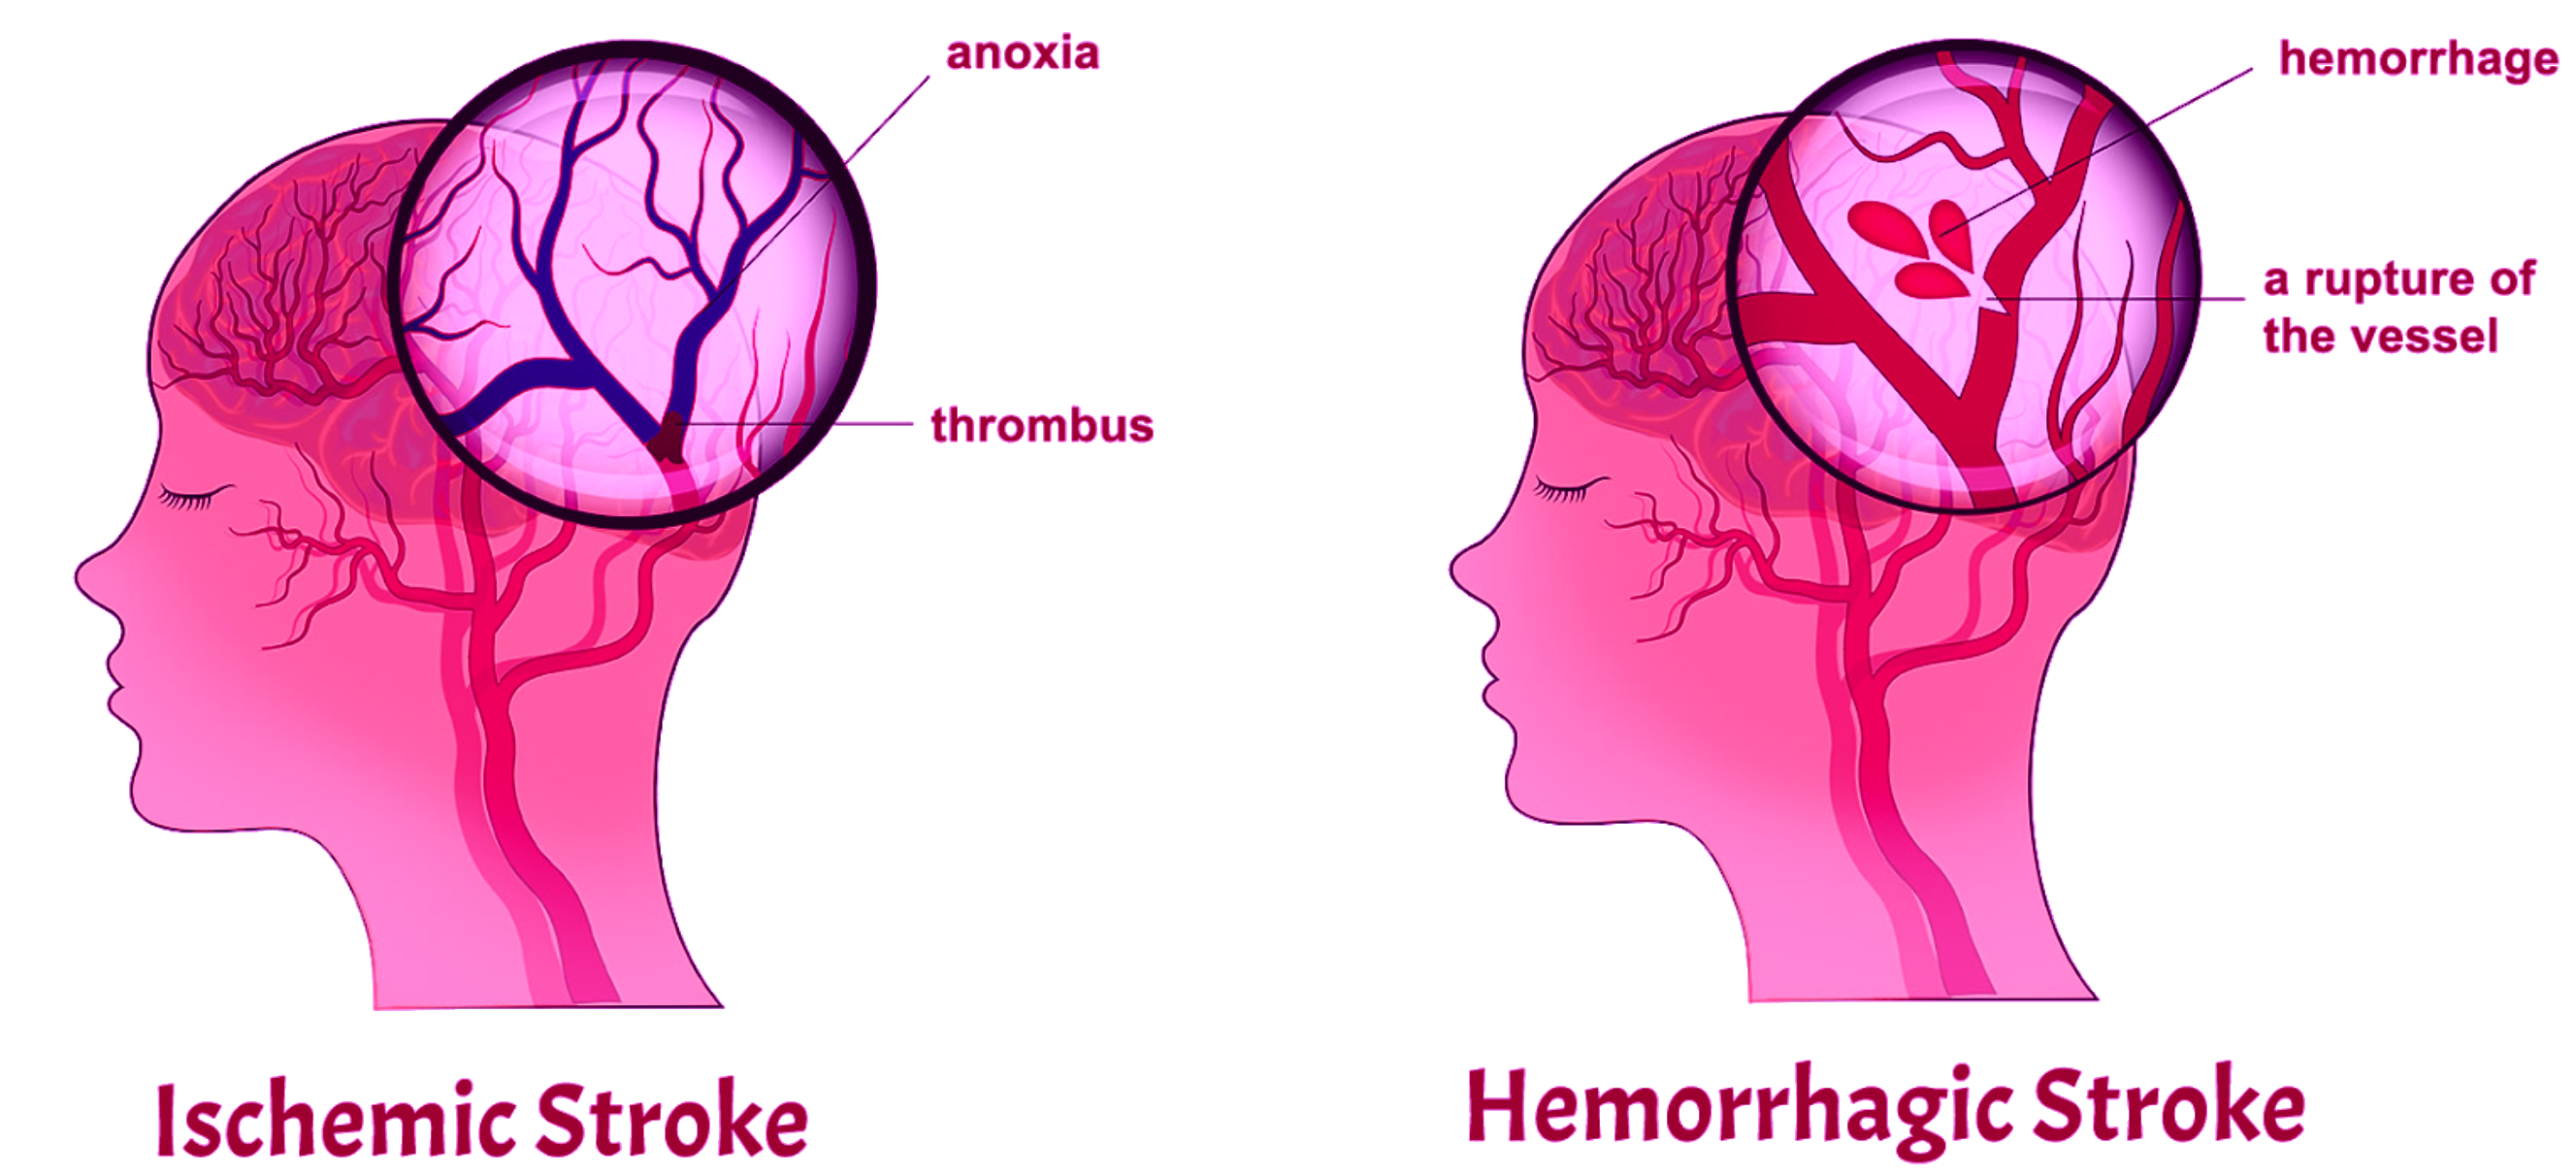
\includegraphics[width=1.0\textwidth]{./images/stroke_types}
\end{center}


\end{frame}
\begin{frame}
\frametitle{Thrombolysis (\emph{'Clot-busting'} medication) in stroke}

While the clot is still fresh, thrombolysis may be given to help break down the clot and restore blood flow.

\vspace{3mm}

\begin{center}
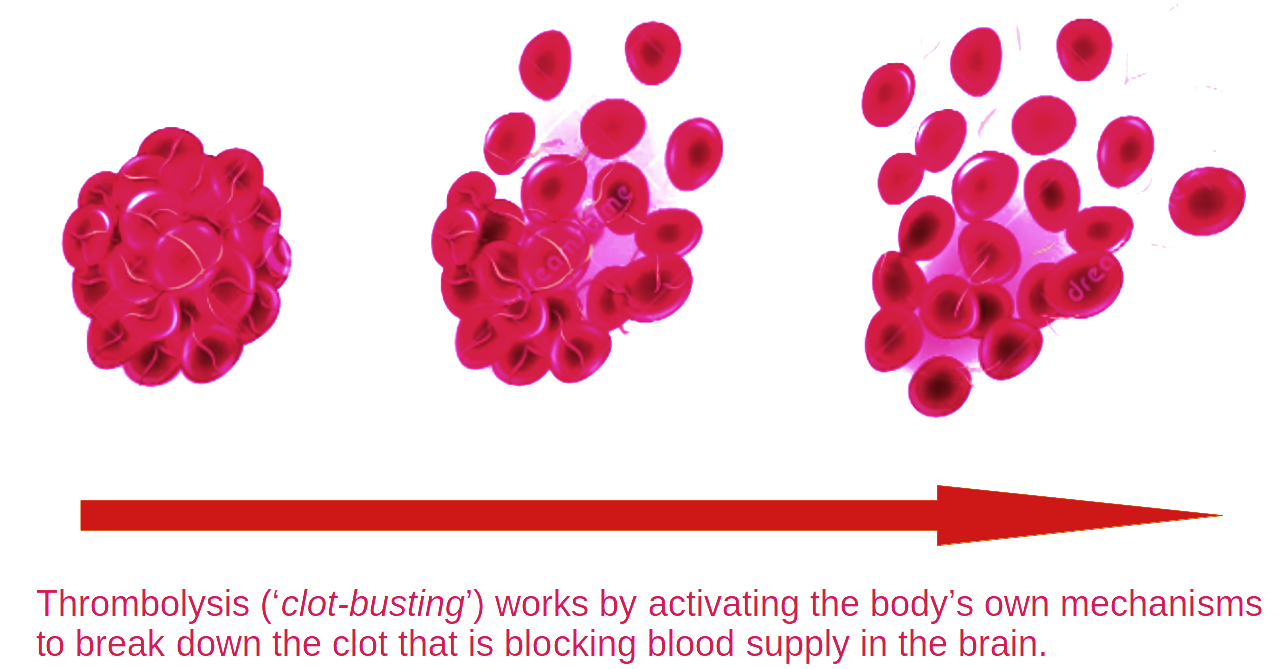
\includegraphics[width=0.70\textwidth]{./images/thrombolysis_mechanism}
\end{center}

\textbf{Drawbacks/limitations}: There is a risk of severe bleed (in about 1 in 50 patients on average, with risk increasing with stroke severity), and thrombolysis loses effectiveness over about the first 5-6 hours.

\end{frame}
\begin{frame}
\frametitle{Use of thrombolysis rates varies significantly between hospitals}

\small
Thrombolysis use varied from below 5\% to 25\% across the 132 acute stroke centres in England and Wales, 2016-2018.
\begin{center}
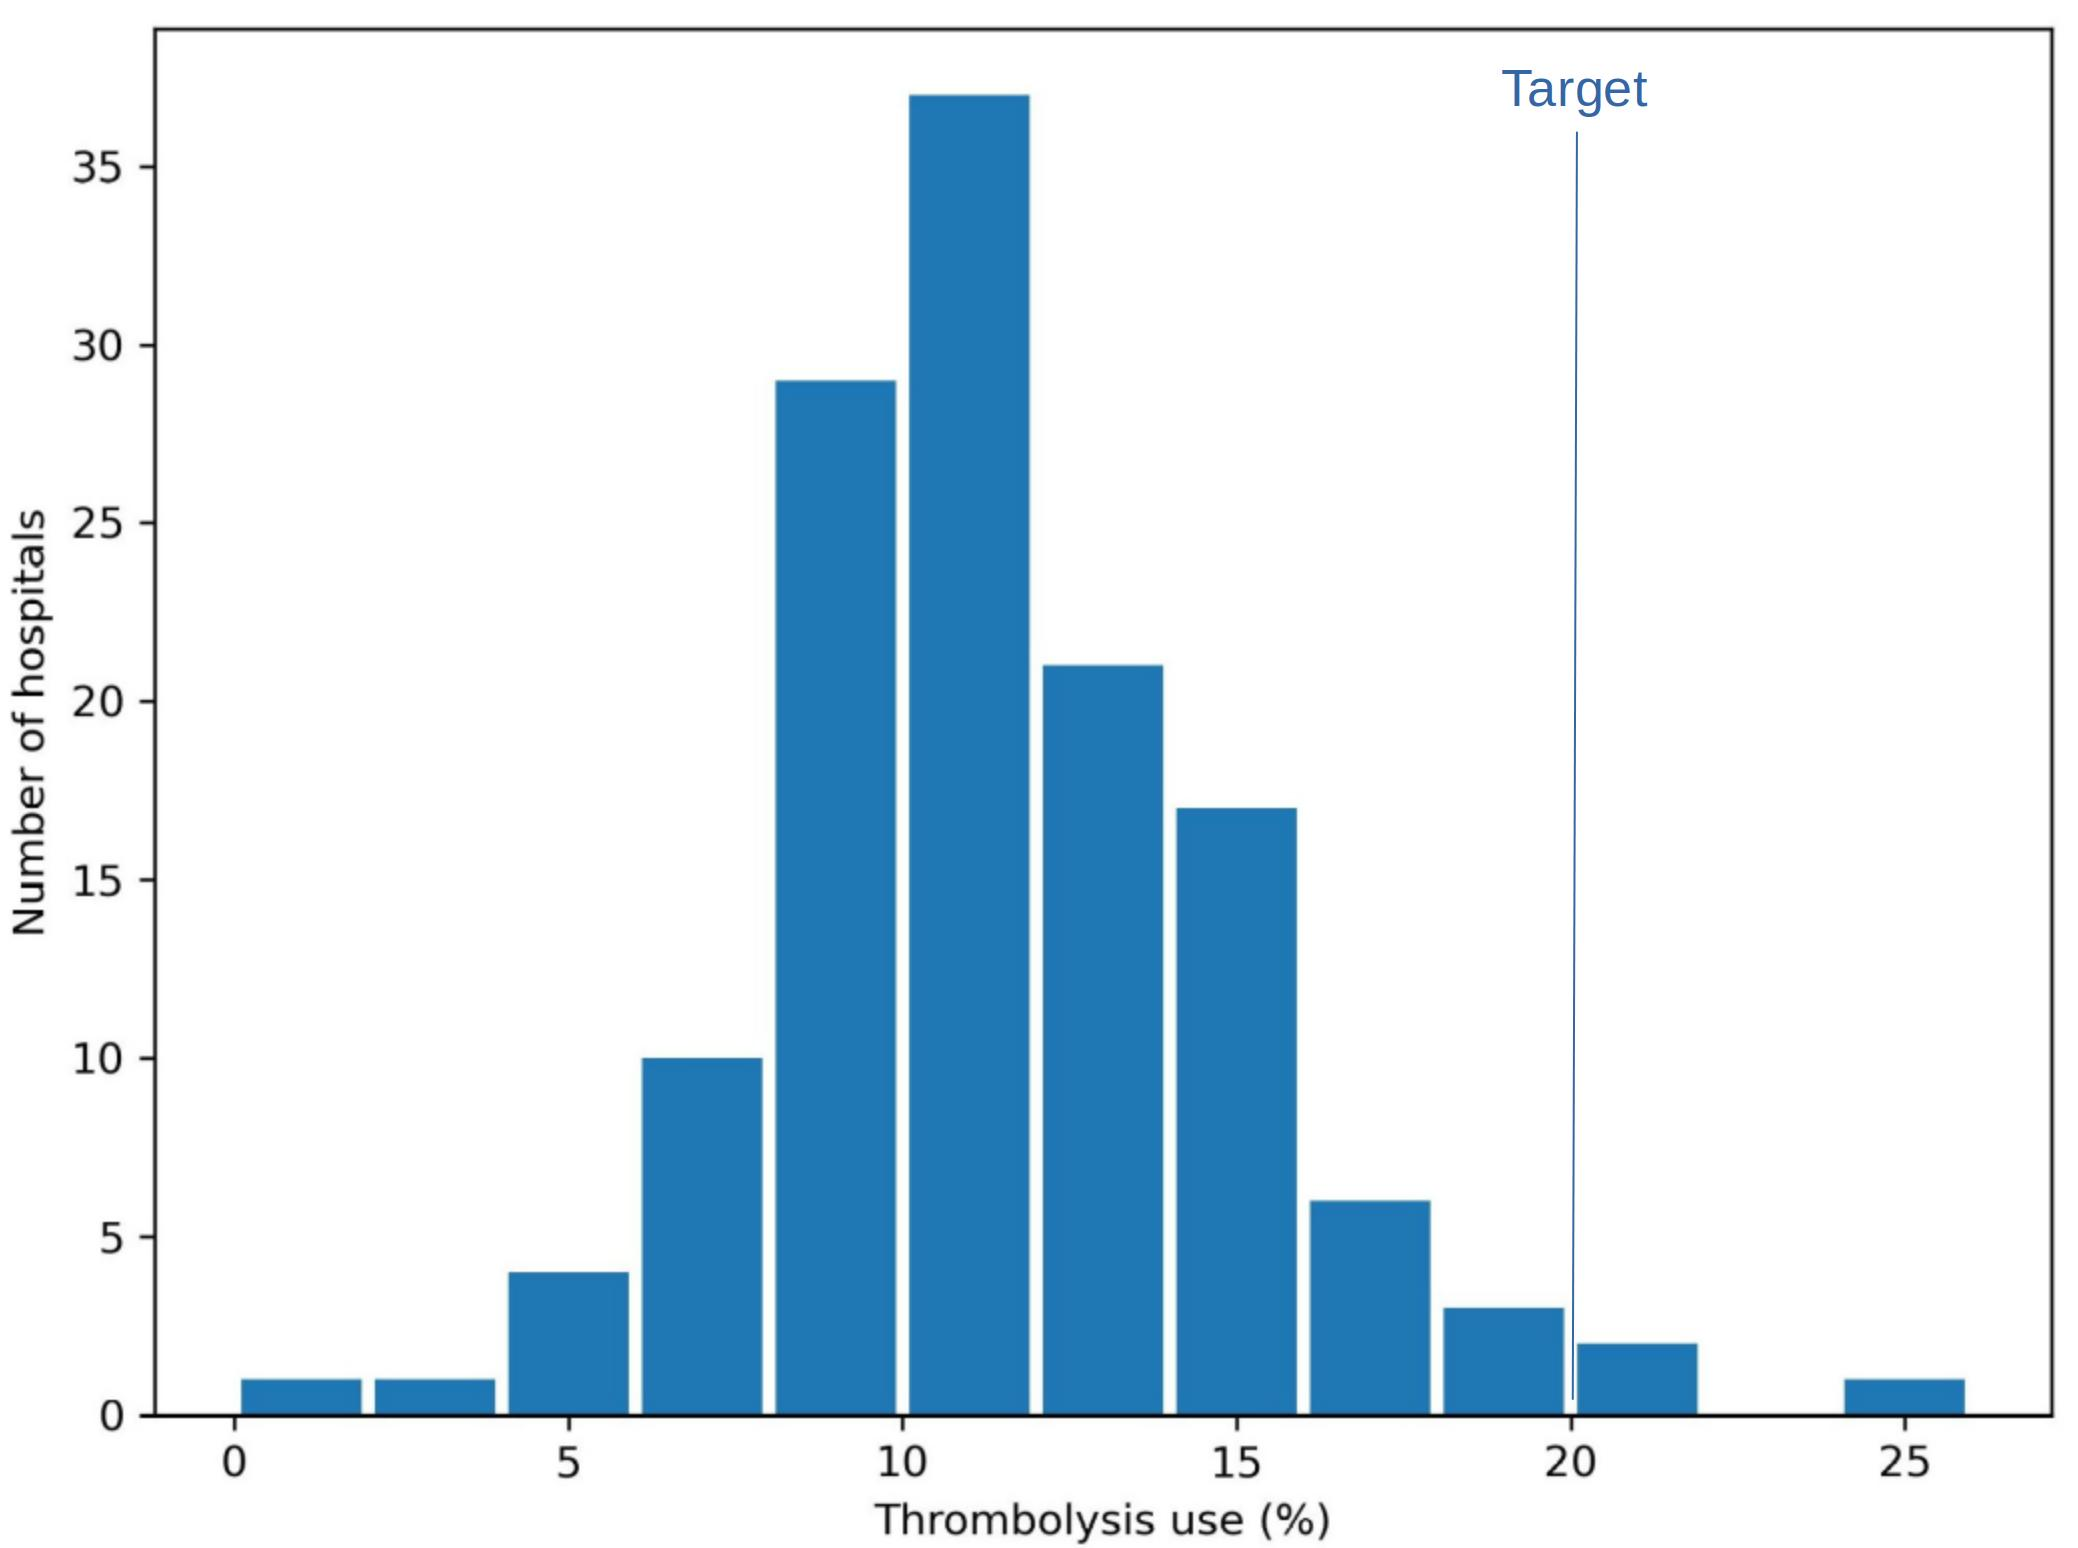
\includegraphics[width=0.50\textwidth]{./images/thrombolysis_by_hospital}
\end{center}

How much of this variation is due to differences in local patient populations, and how much is due to differences in in-hospital processes and decisions hospitals make on who they would give thrombolysis to?
\end{frame}
\begin{frame}
\frametitle{Breaking down the emergency stroke pathway into key steps}
\begin{center}
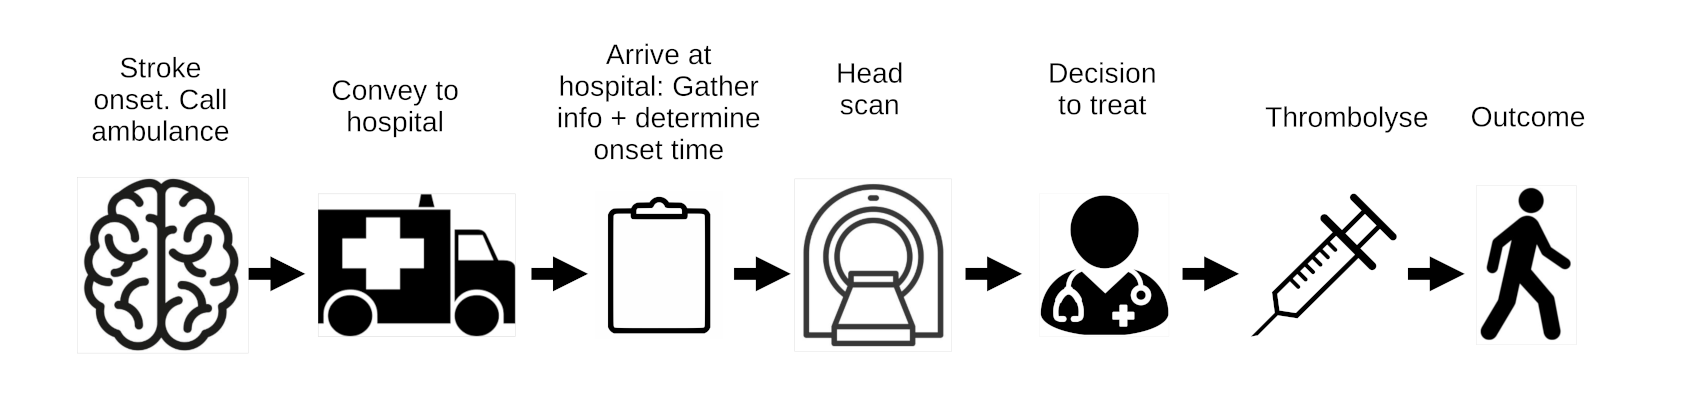
\includegraphics[width=1.0\textwidth]{./images/pathway}
\end{center}
We can model key changes to pathway, such as:
\begin{small}
\begin{itemize}
    \item What if the pathway were \textbf{faster}?
    \item What if hospital \textbf{determined the stroke onset time} in more patients?
    \item What if clinical \textbf{decision-making} was like that of \emph{benchmark} hospitals? (Predict what treatment a patient would receive at other hospitals).
\end{itemize}
\end{small}
\footnotesize{We model these changes with a hospital's own patient population, to allow for inter-hospital variation in patient population characteristics.}
\end{frame}
\begin{frame}
\frametitle{Our Approach}

\small

\begin{itemize}
    \item Train a machine learning algorithm to learn to predict to which patients each hospital would, or would not, give thrombolysis.
    \item Identify the patient characteristics which are most important in predicting use of thrombolysis, and produce a simpler machine learning model based on these characteristics.
    \item Identify \emph{ideal} candidates for thrombolysis.
    \item Add an \emph{explainable machine learning} layer* to understand patterns of use of thrombolysis.
    \item Investigate what we think would happen if every hospital received exactly the same 10k cohort of patients.
    \item Identify key subgroups of patients where hospitals differ in their use of thrombolysis.
\end{itemize}

\vspace{3mm}
\footnotesize
*SHAP (Shapley Additive Values, which provide information on what contribution each patient characteristic makes to the final prediction of whether they will, or will not, receive thrombolysis).
\end{frame}
\begin{frame}
\frametitle{Machine learning overview}
\begin{center}
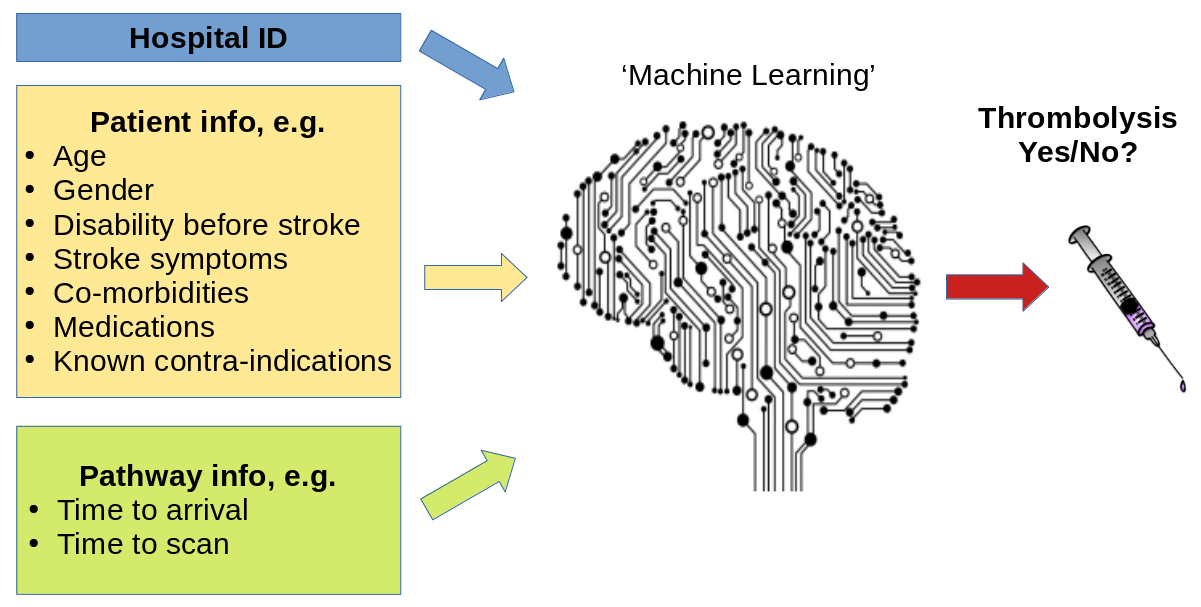
\includegraphics[width=0.80\textwidth]{./images/ml_model_high_level}
\end{center}

\small
\textbf{Machine learning is based on the simple principle of recognising similarity to what has been seen before.}
\vspace{2mm}

\footnotesize{We accessed 246,676 emergency stroke admissions in England and Wales over three years. Our machine learning models use XGBoost classification, and are based on those 88,928 patients who arrive within 4 hours of known stroke onset. Accuracy = 85\% (ROC AUC = 0.92).}
\end{frame}
\begin{frame}
\frametitle{XGBoost algorithm}

\begin{itemize}
    \small
    \item We used the XGBoost  (eXtreme Gradient Boosting) algorithm. It works by combining multiple weak predictive models to  create a stronger, more accurate model.
    \item XGboost uses multiple decision trees, each of which is built to reduce the residual error from the previous tree.
    \item The weight of each tree reduces as trees are added (to avoid over-fitting).
    \item The final prediction is the sum of the predictions of all the trees multiplied by their weights.

\end{itemize}

\begin{center}
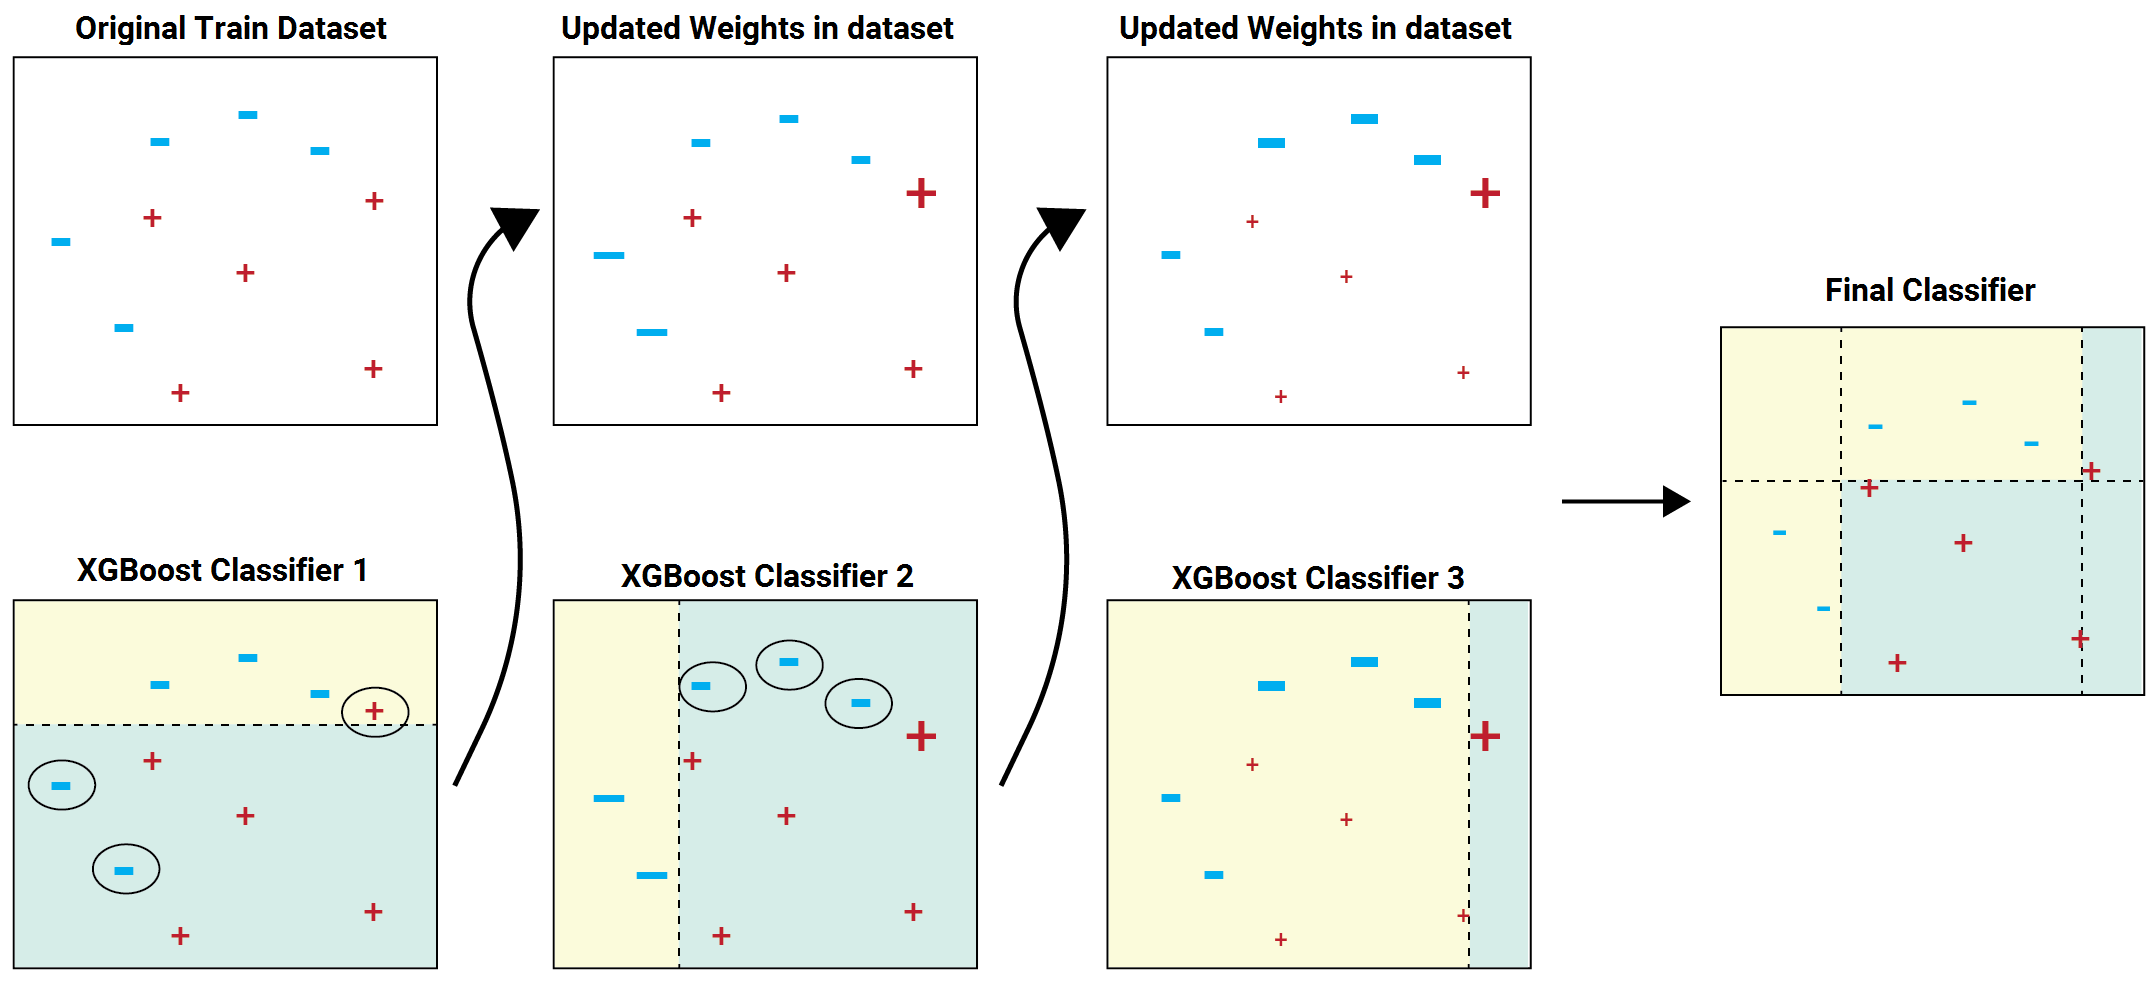
\includegraphics[width=0.75\textwidth]{./images/xgboost}
\end{center}

\tiny
Image from \url{https://blog.quantinsti.com/xgboost-python/}

\end{frame}
\begin{frame}{Model accuracy, and simplification}

A model with all available 84 features had an ROC AUC of 0.922. A model with 10 features had an ROC AUC of 0.919.

\begin{center}
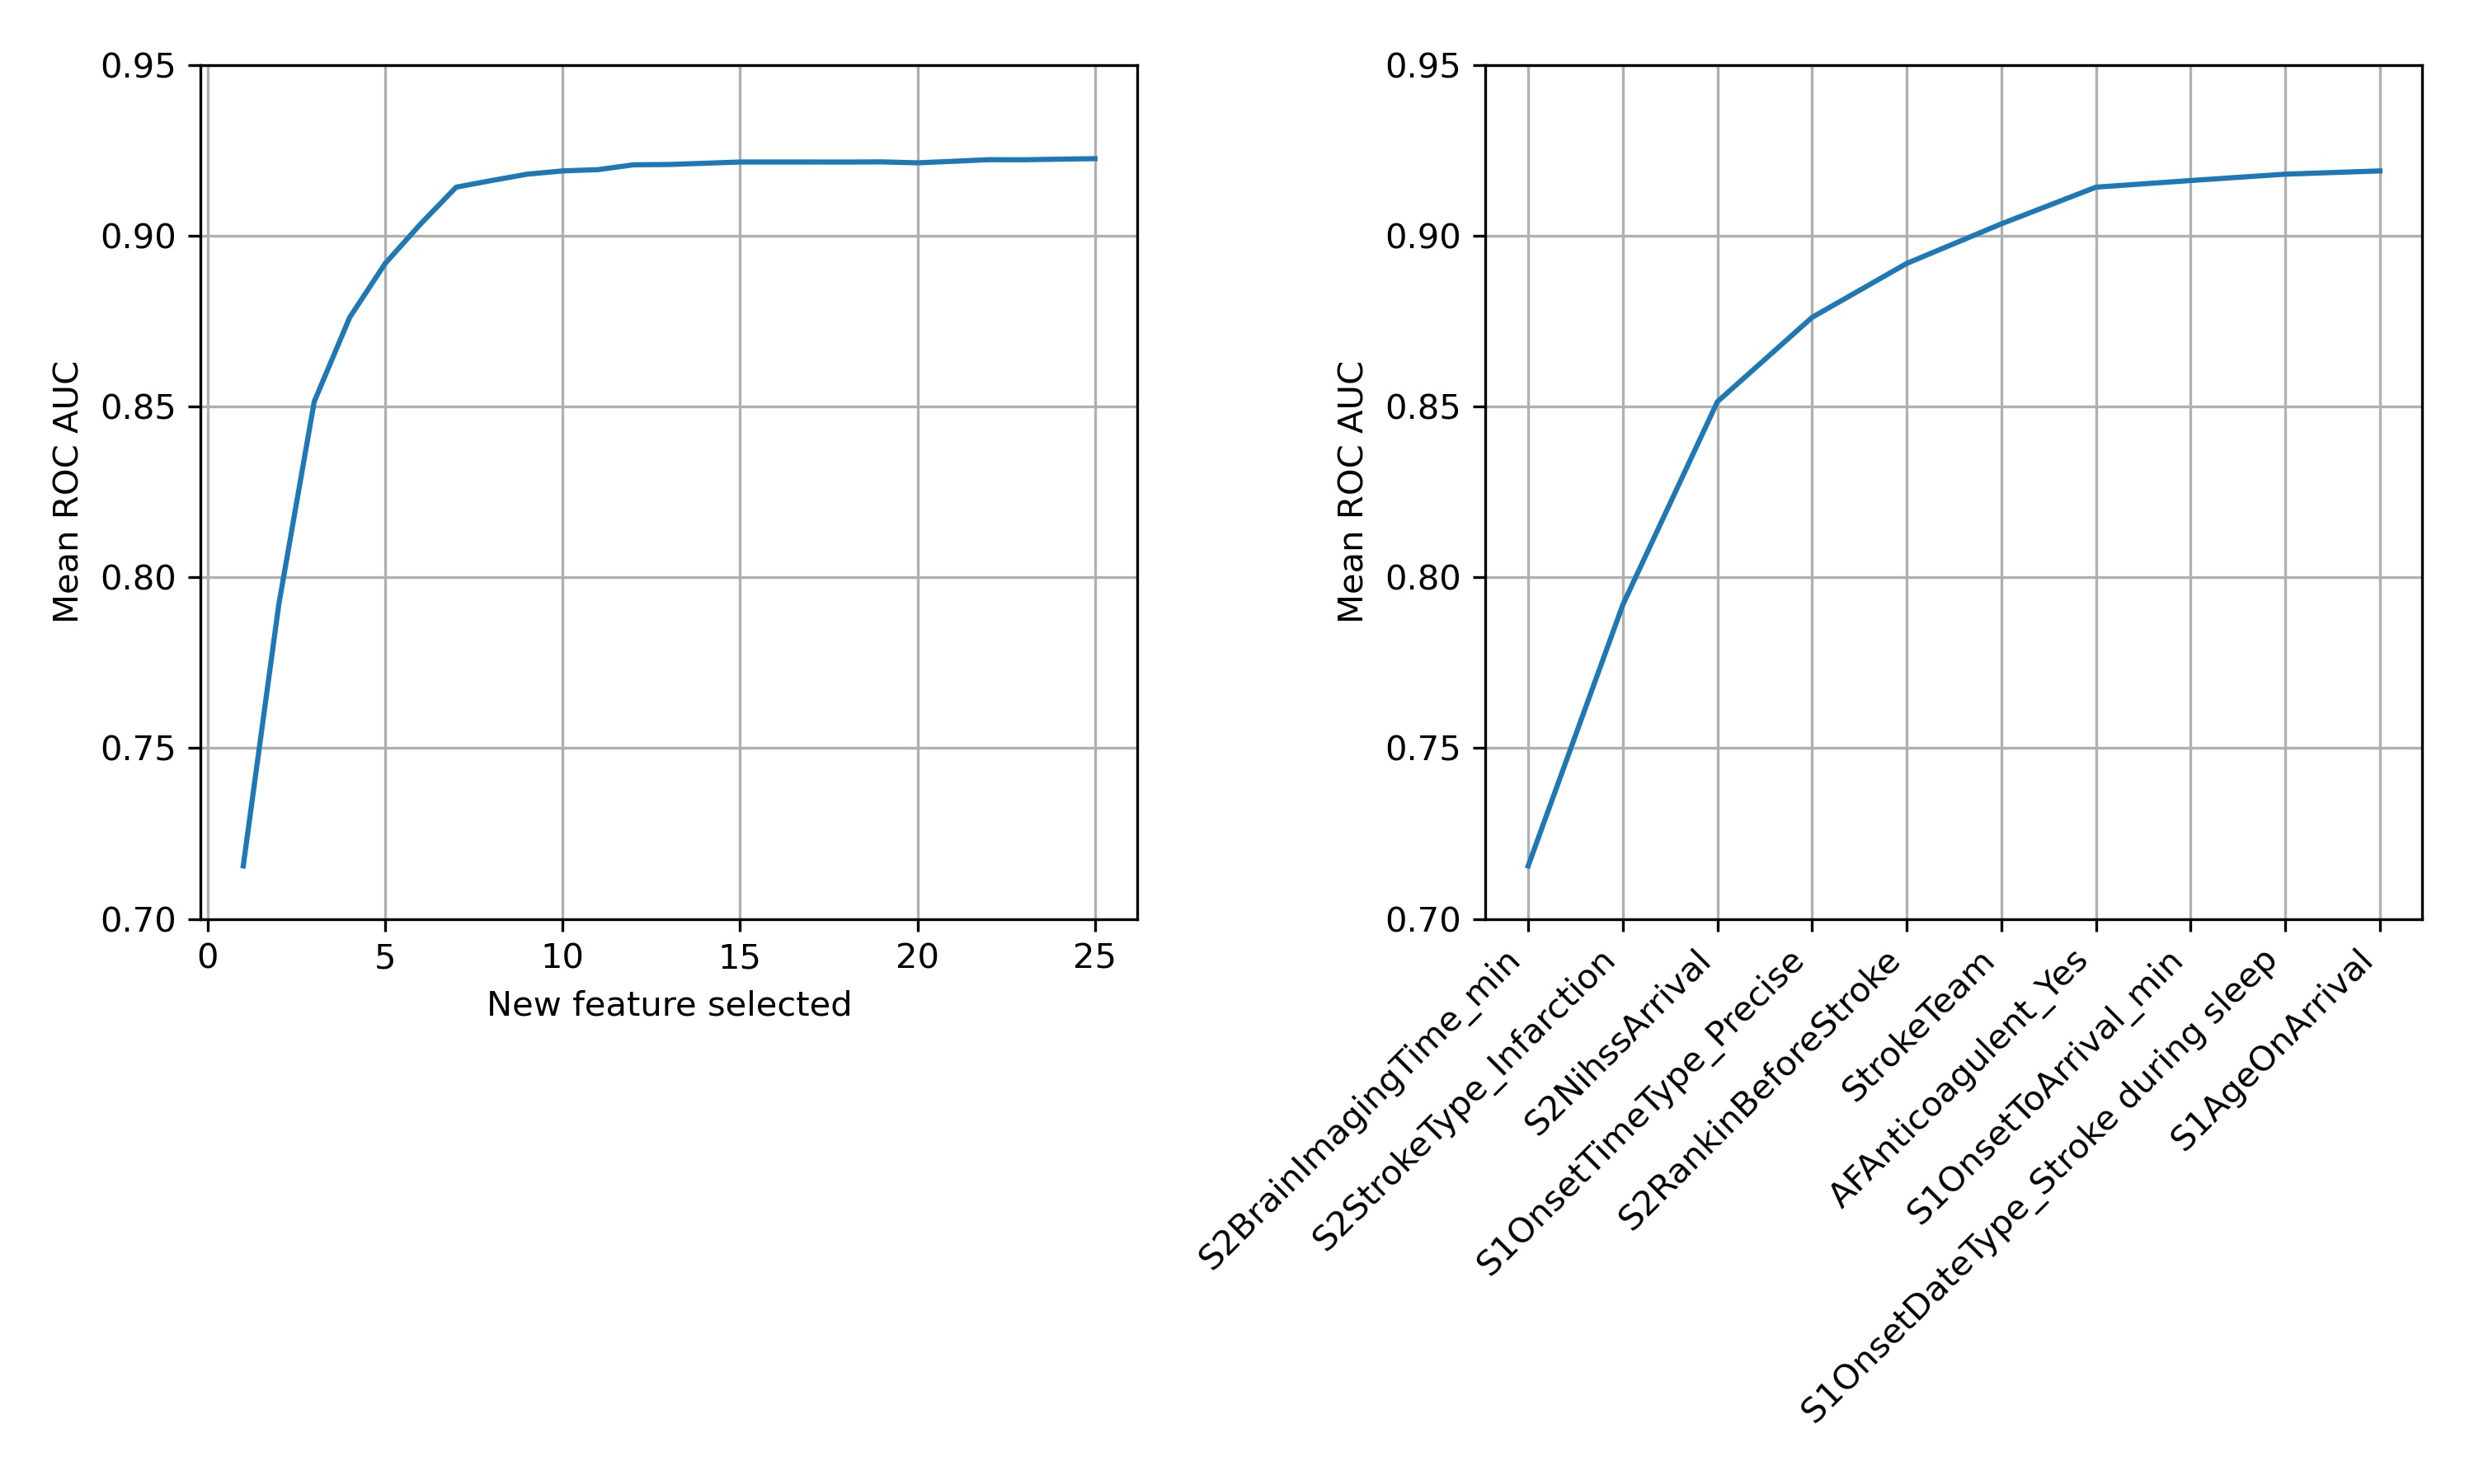
\includegraphics[width=0.9\textwidth]{./images/01_feature_selection.jpg}
\end{center}

Our simpler machine learning model will just use these 10 features.

\end{frame}
\begin{frame}{Predicting hospital thrombolysis use}

Predicted thrombolysis use was measured by combining 5 test sets from k-fold validation. The predicted vs. observed thrombolysis are highly correlated (r-squared 0.977). 

\begin{center}
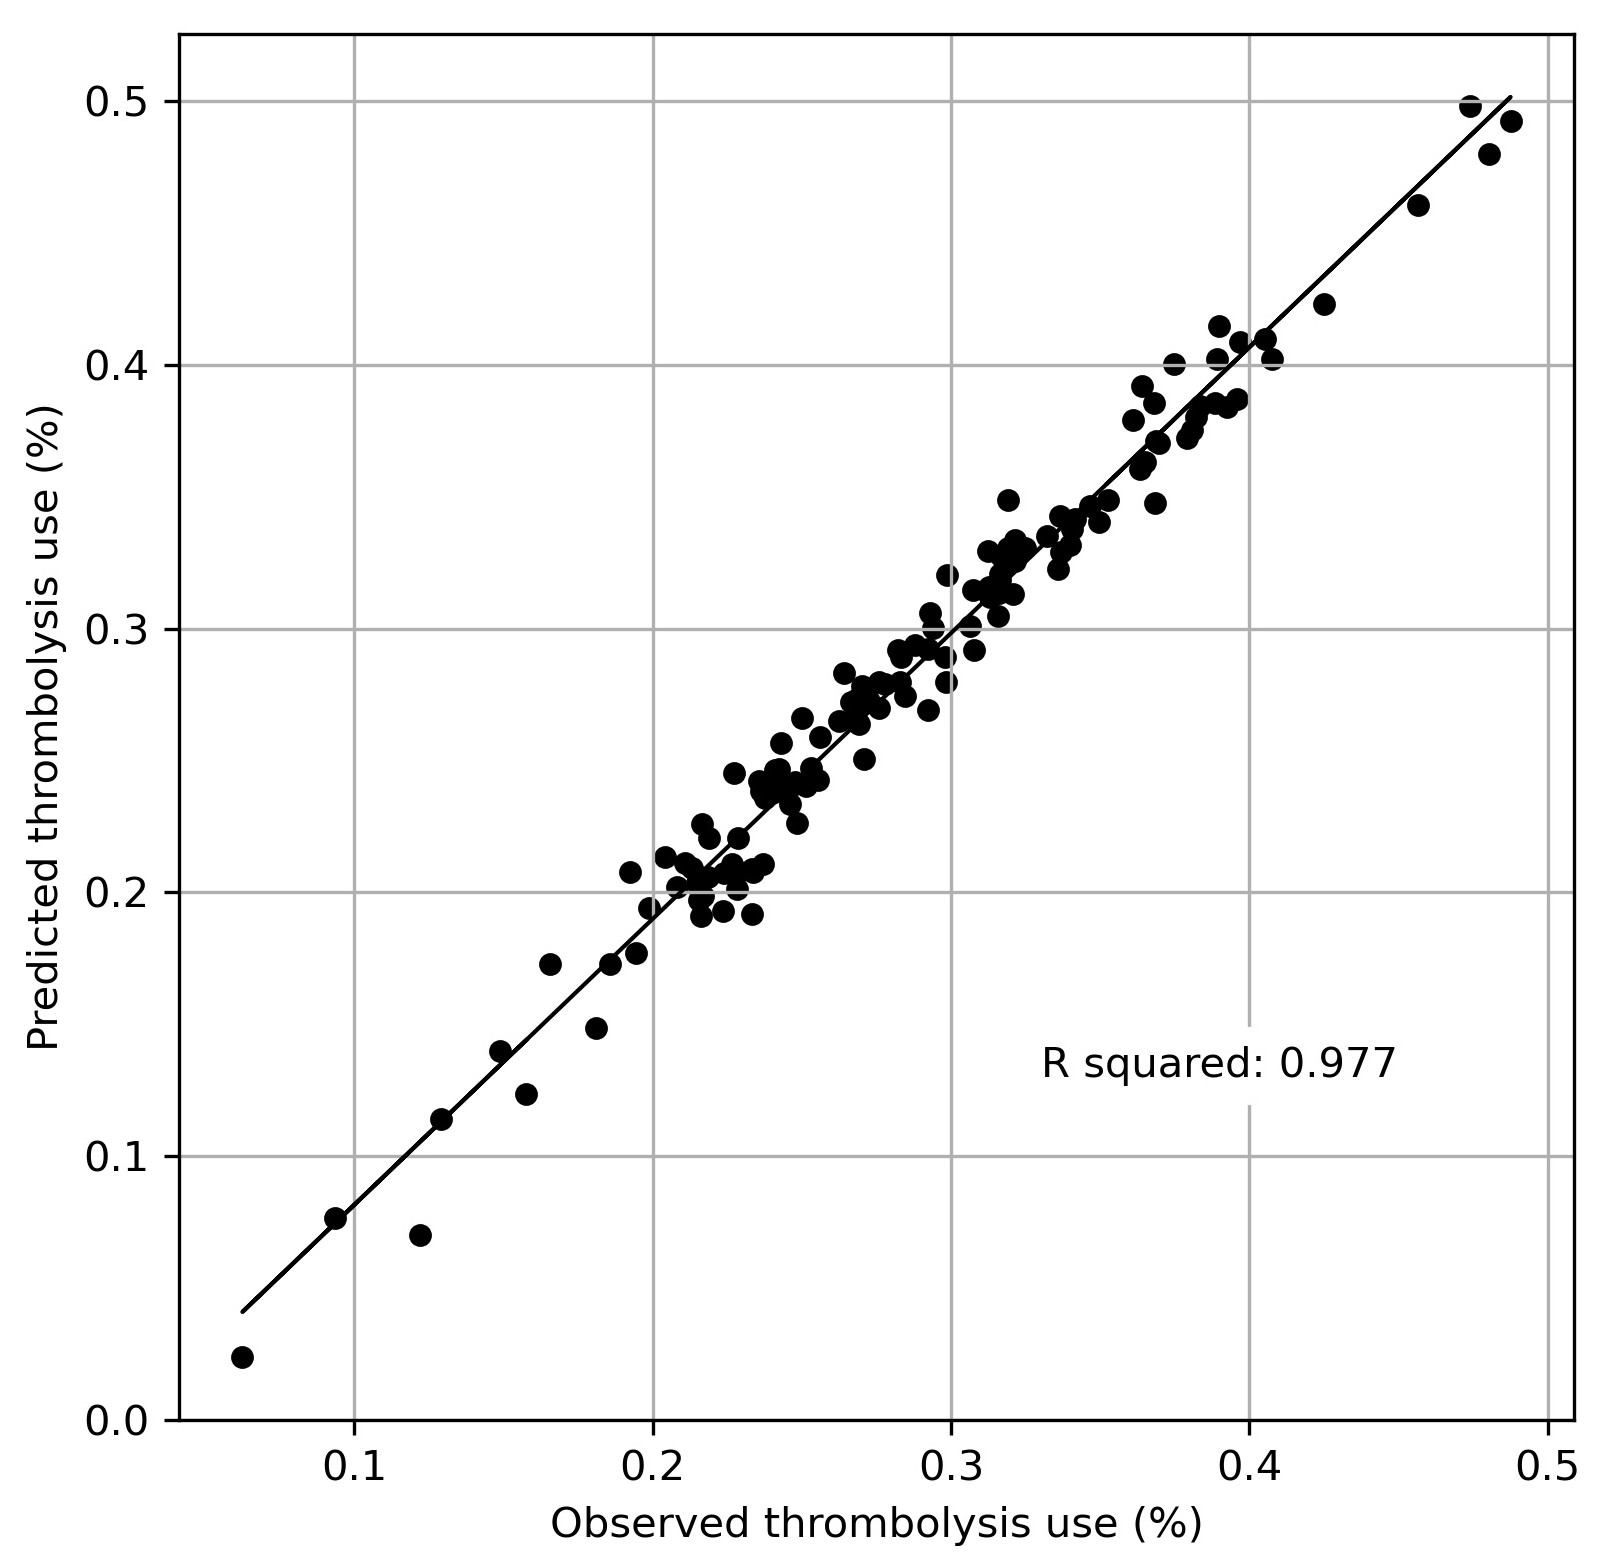
\includegraphics[width=0.55\textwidth]{./images/02_xgb_10_features_observed_predicted_rates.jpg}
\end{center}



\end{frame}
\begin{frame}
\frametitle{Explaining model predictions with SHAP values}

SHAP values show the influence of features (even for \emph{`black box'} models).

\begin{center}
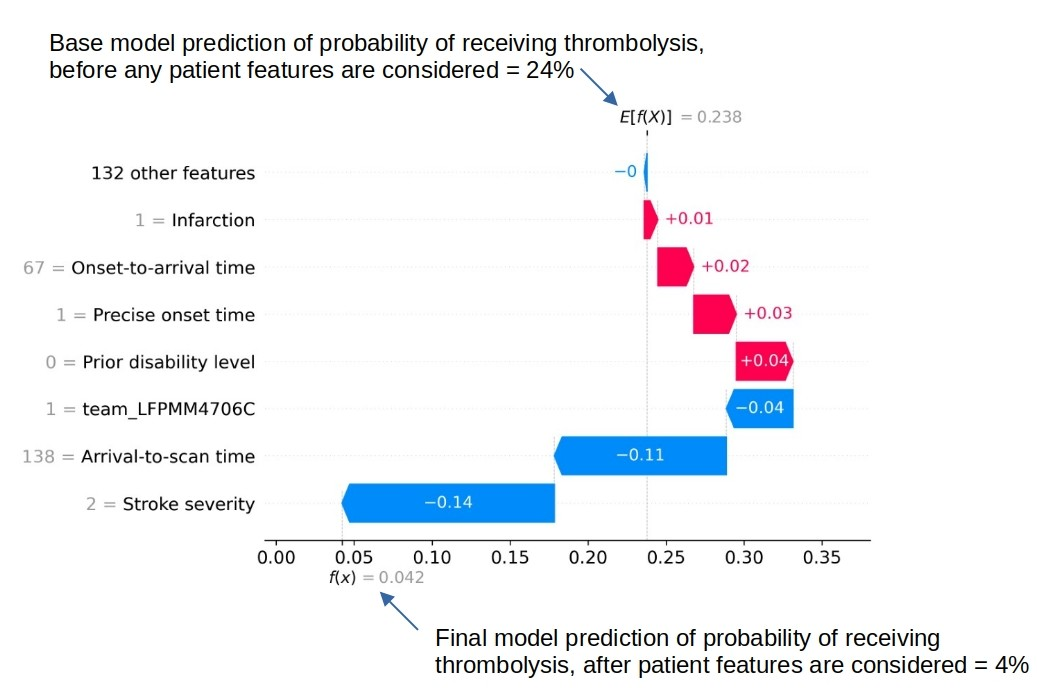
\includegraphics[width=0.90\textwidth]{./images/xgb_waterfall_low_probability_2.jpg}
\end{center}
\end{frame}
\begin{frame}
\frametitle{SHAP values for thrombolysis prediction}
Note: SHAP values here are log odds. 
\begin{center}
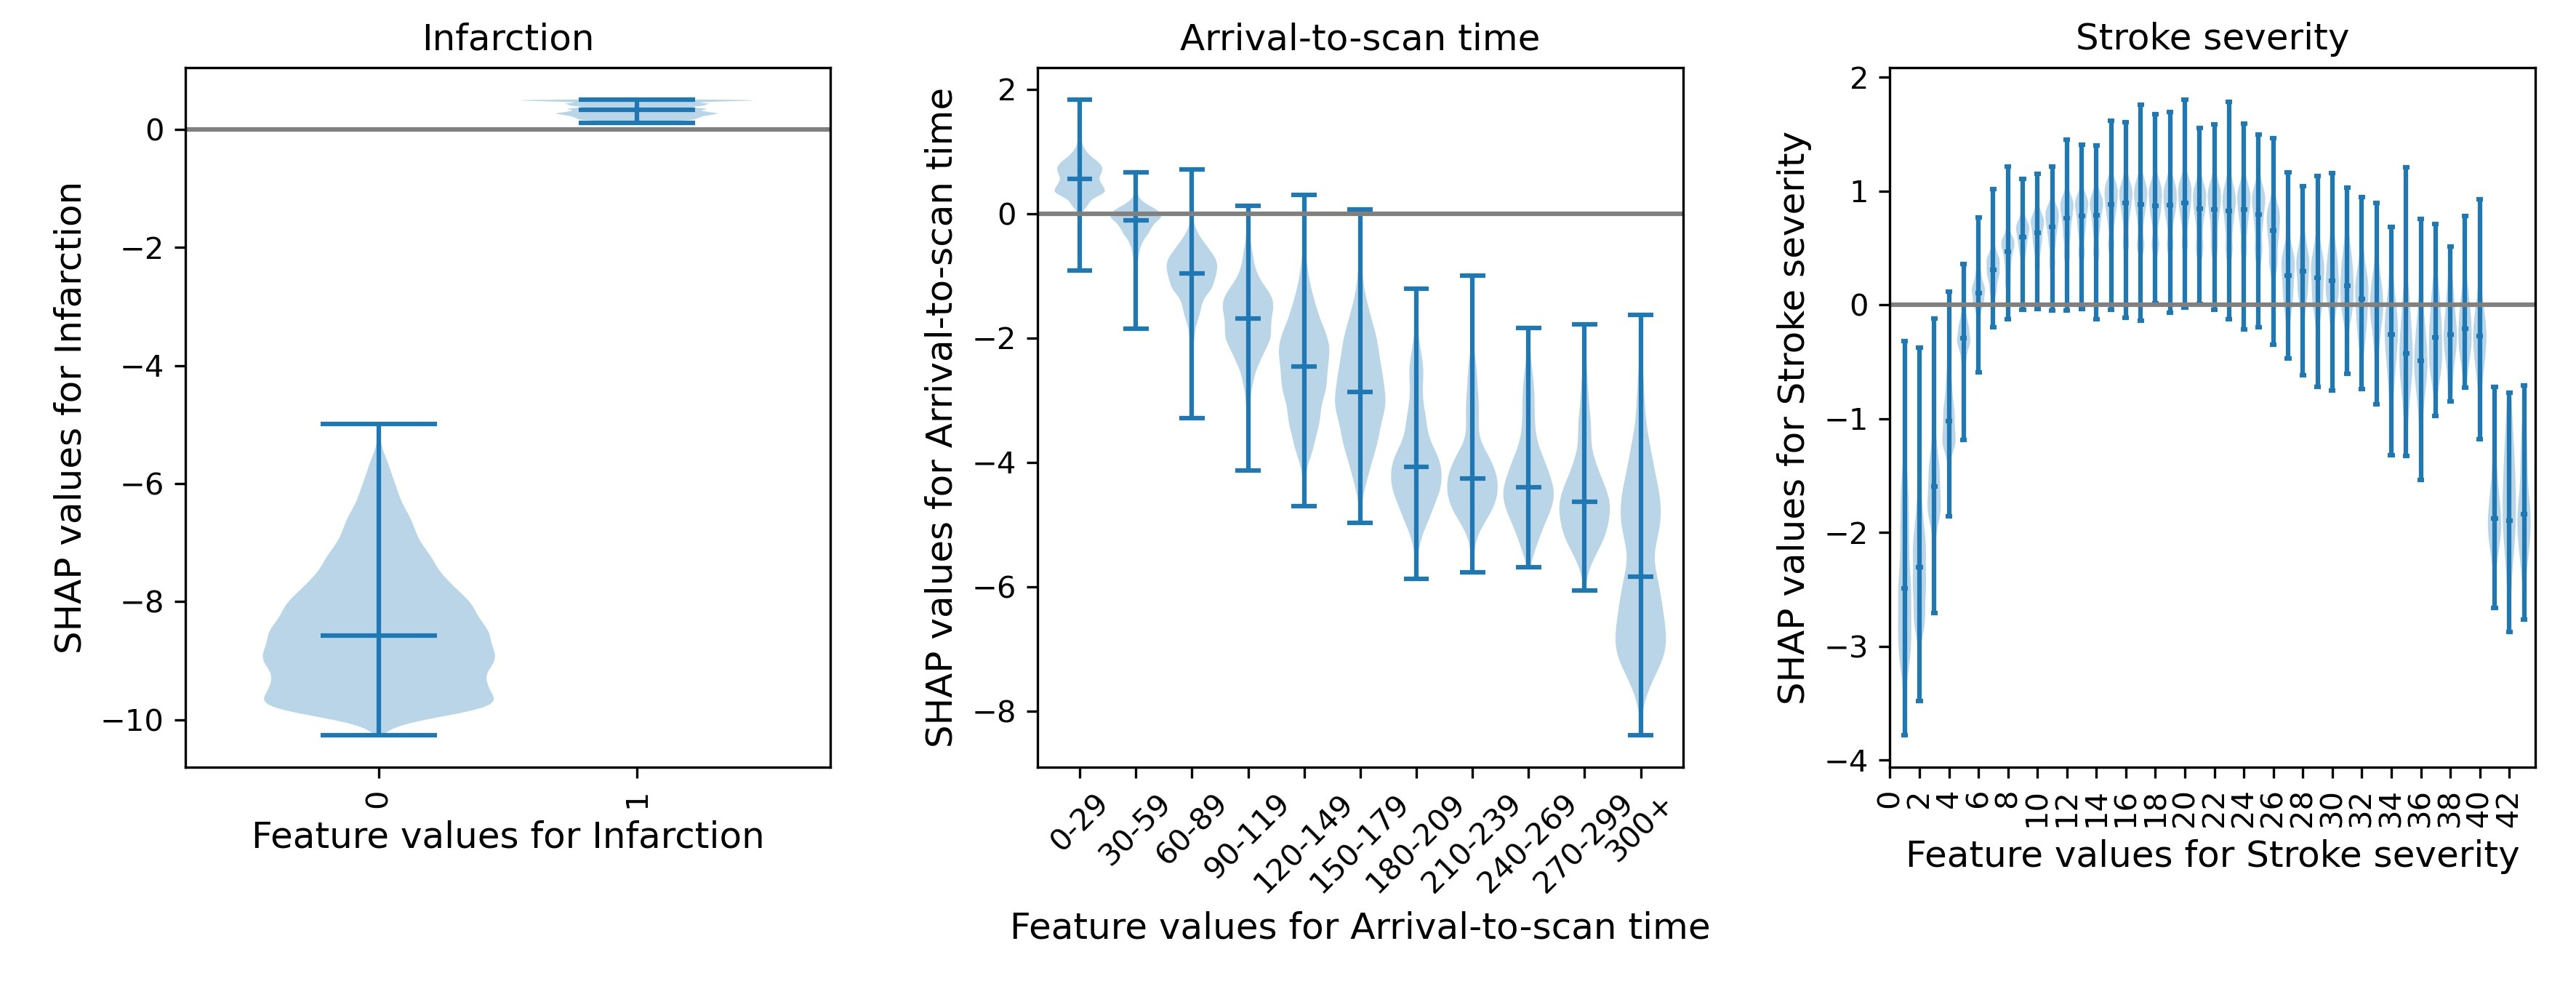
\includegraphics[width=1.0\textwidth]{./images/03d_xgb_10_features_thrombolysis_shap_violin_1.jpg}
\end{center}

\scriptsize
SHAP effects: \\
$\pm1$: Odds change $\pm3$ fold\\
$\pm2$: Odds change $\pm7$ fold\\
$\pm3$: Odds change $\pm20$ fold\\
$\pm4$: Odds change $\pm55$ fold\\
$\pm5$: Odds change $\pm150$ fold
\end{frame}
%\begin{frame}
\frametitle{SHAP values for each feature - 2}
Note: SHAP values here are log odds. 
\begin{center}
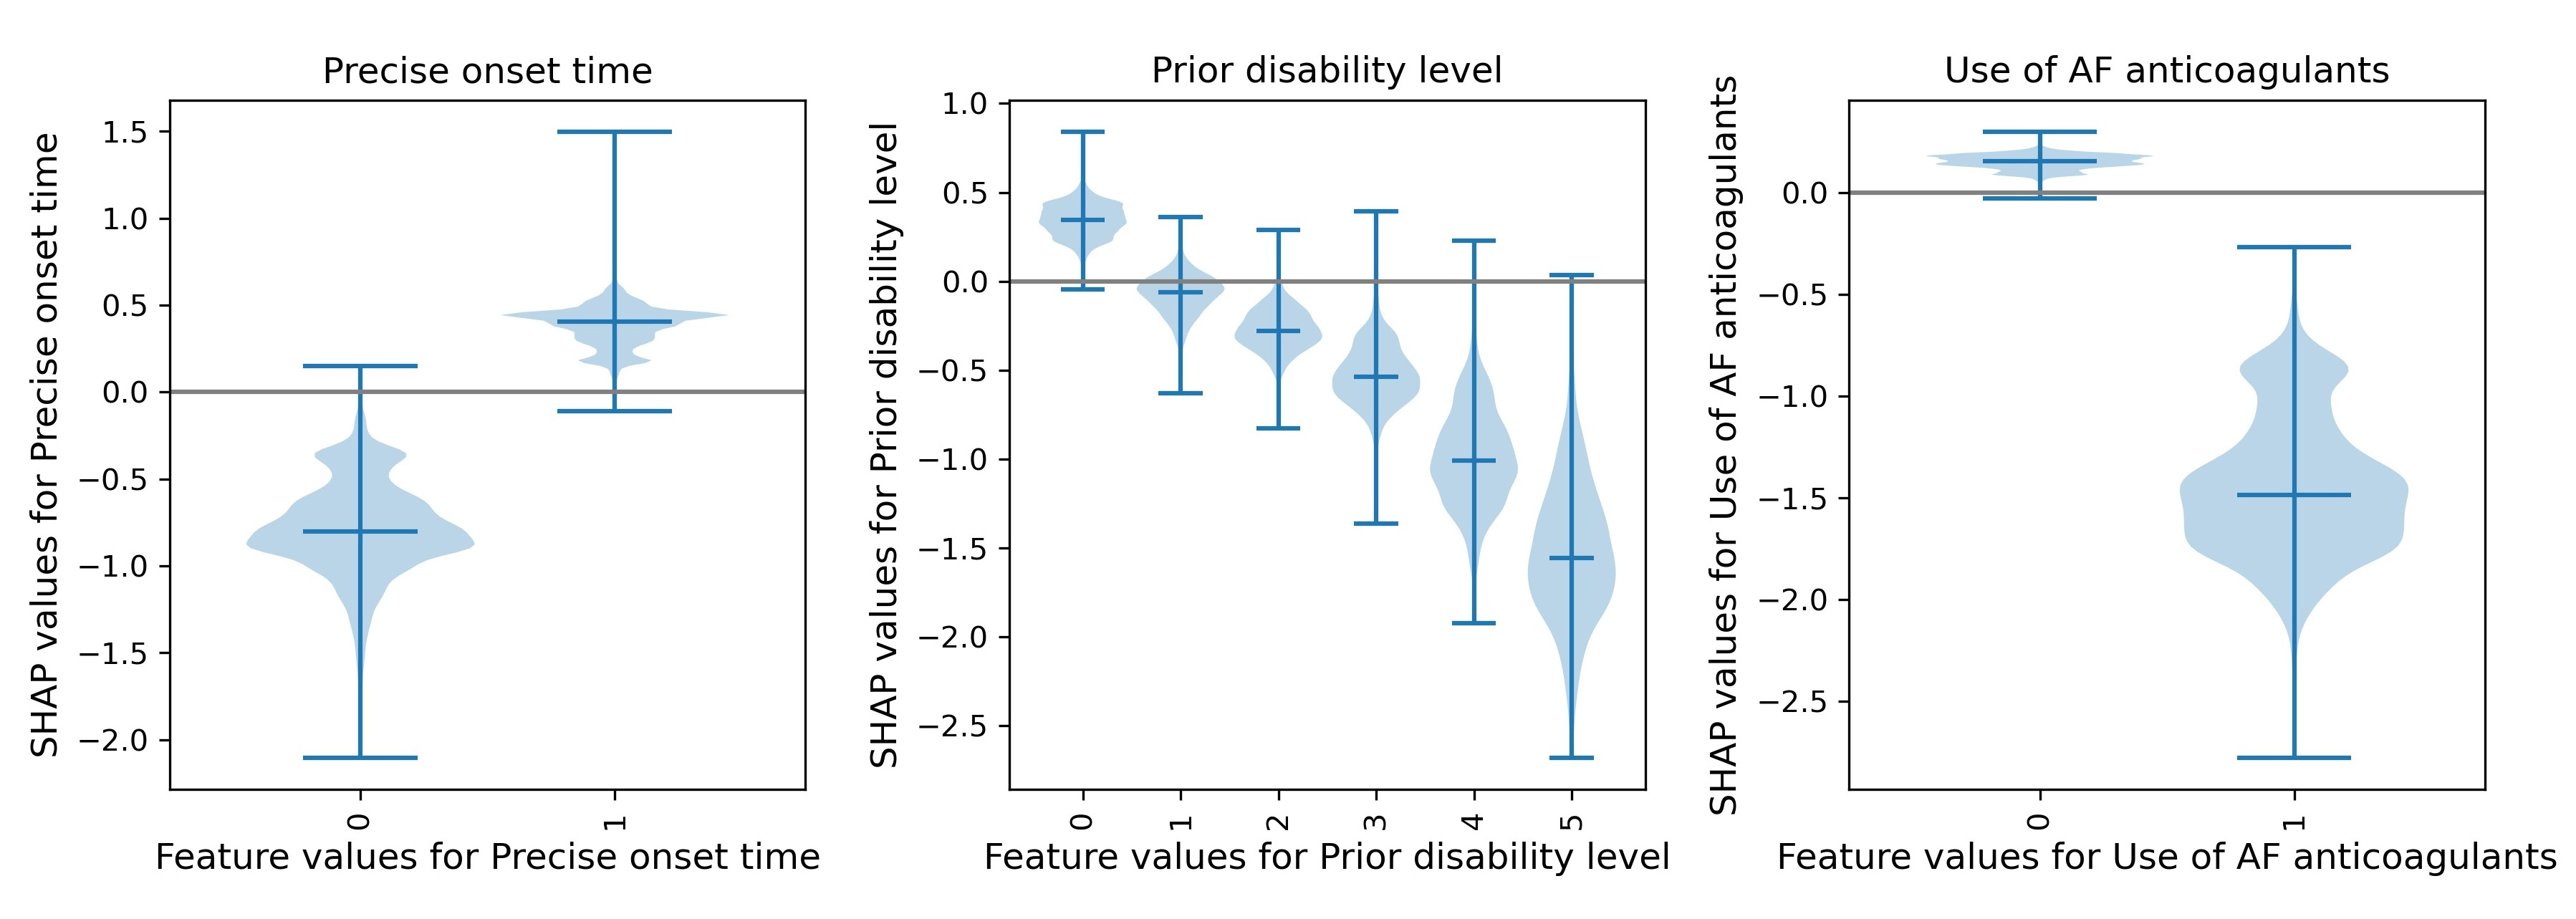
\includegraphics[width=1.0\textwidth]{./images/03d_xgb_10_features_thrombolysis_shap_violin_2.jpg}
\end{center}
\scriptsize
SHAP effects: \\
$\pm1$: Odds change $\pm3$ fold\\
$\pm2$: Odds change $\pm7$ fold\\
$\pm3$: Odds change $\pm20$ fold\\
$\pm4$: Odds change $\pm55$ fold\\
$\pm5$: Odds change $\pm150$ fold
\end{frame}
%\begin{frame}
\frametitle{SHAP values for each feature - 3}
Note: SHAP values here are log odds. 
\begin{center}
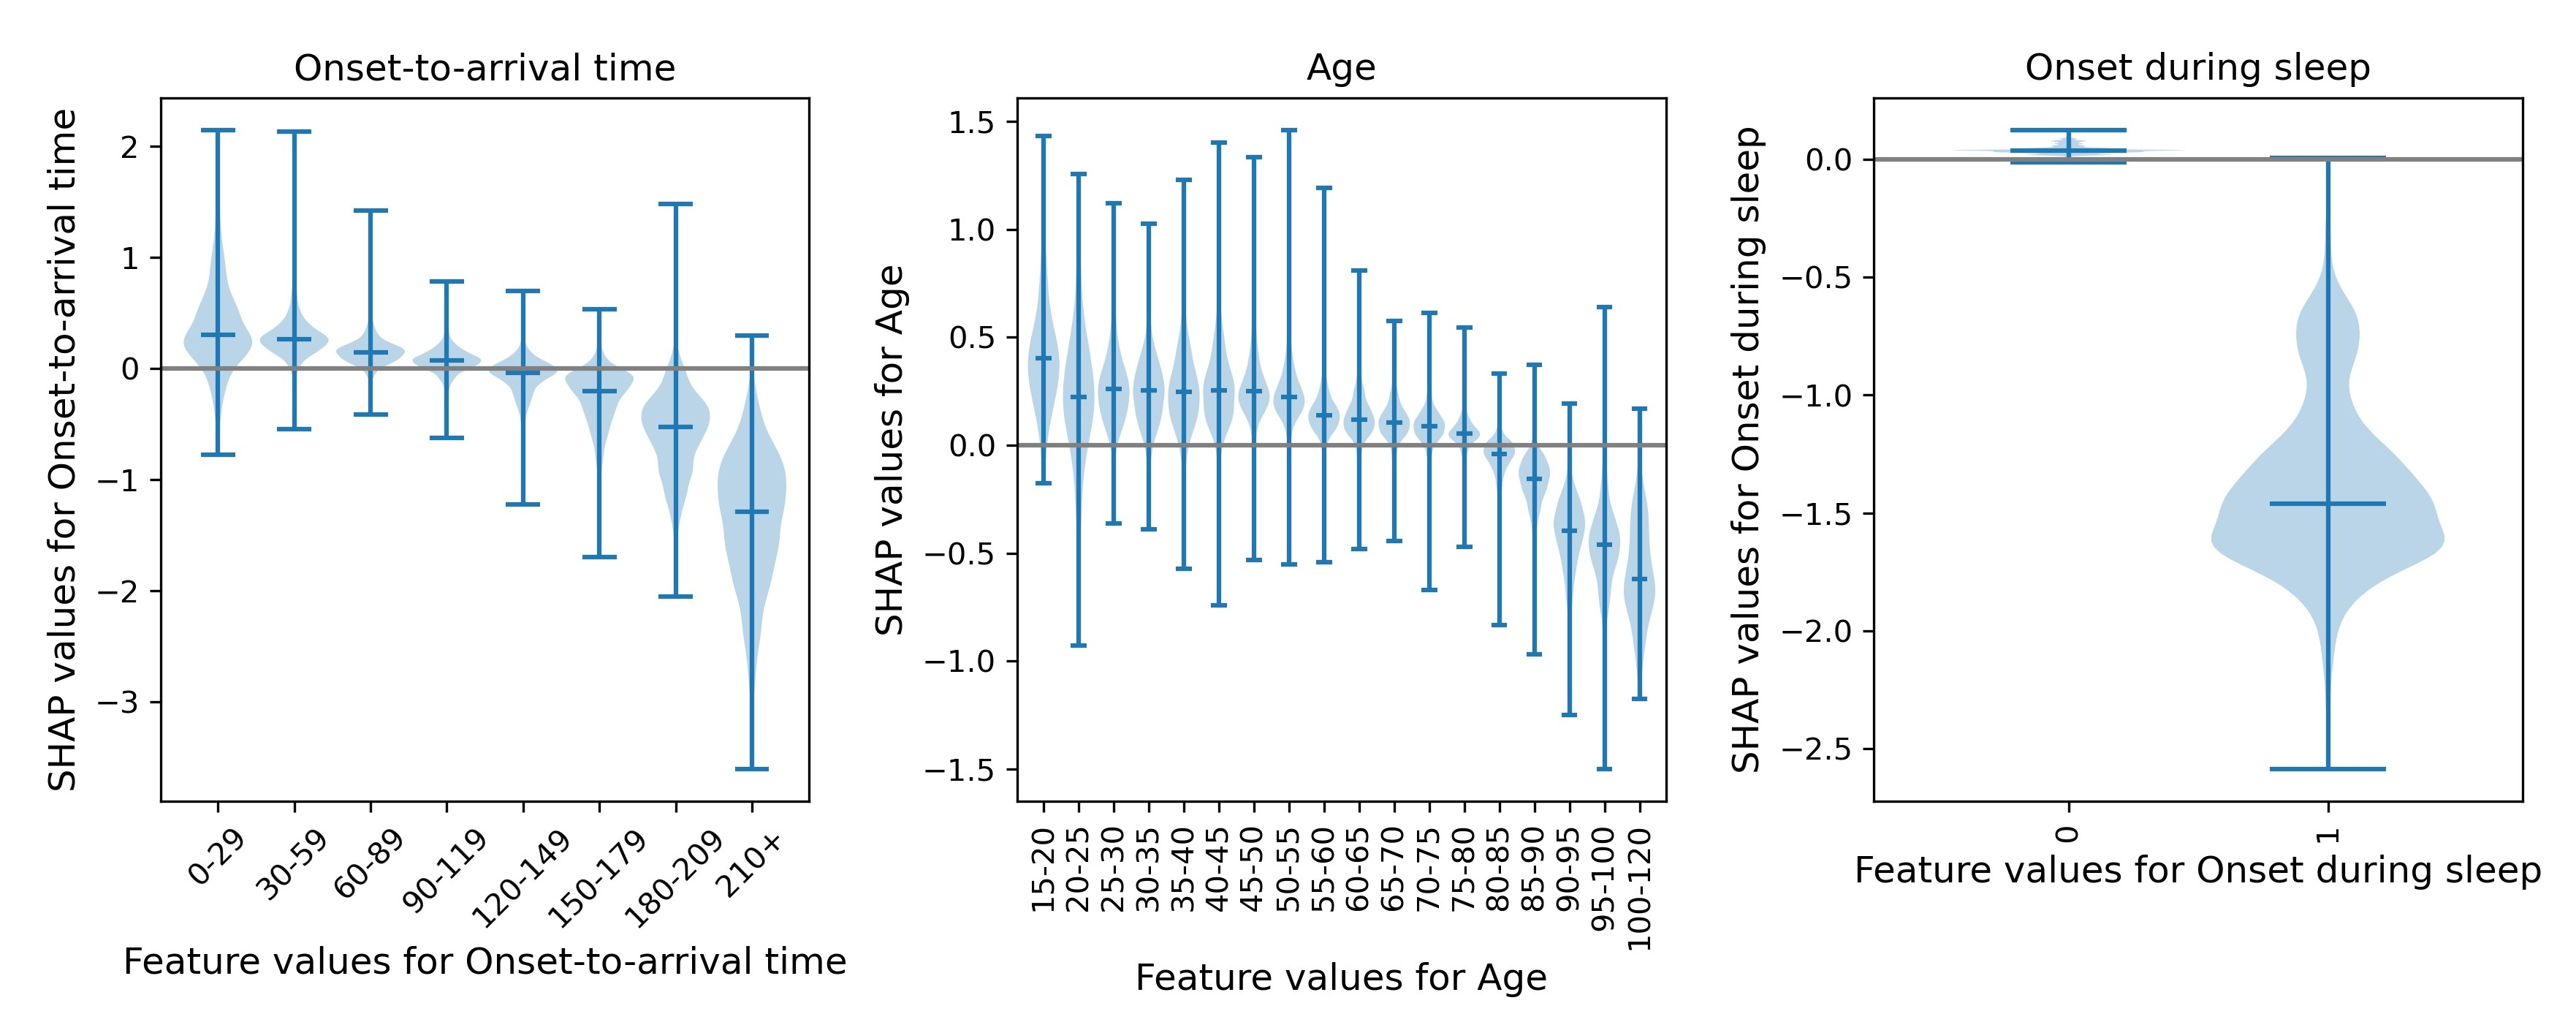
\includegraphics[width=1.0\textwidth]{./images/03d_xgb_10_features_thrombolysis_shap_violin_3.jpg}
\end{center}
\scriptsize
SHAP effects: \\
$\pm1$: Odds change $\pm3$ fold\\
$\pm2$: Odds change $\pm7$ fold\\
$\pm3$: Odds change $\pm20$ fold\\
$\pm4$: Odds change $\pm55$ fold\\
$\pm5$: Odds change $\pm150$ fold
\end{frame}
\begin{frame}
\frametitle{Isolating the effect of hospitals}
Note: SHAP values here are log odds. 
\begin{center}
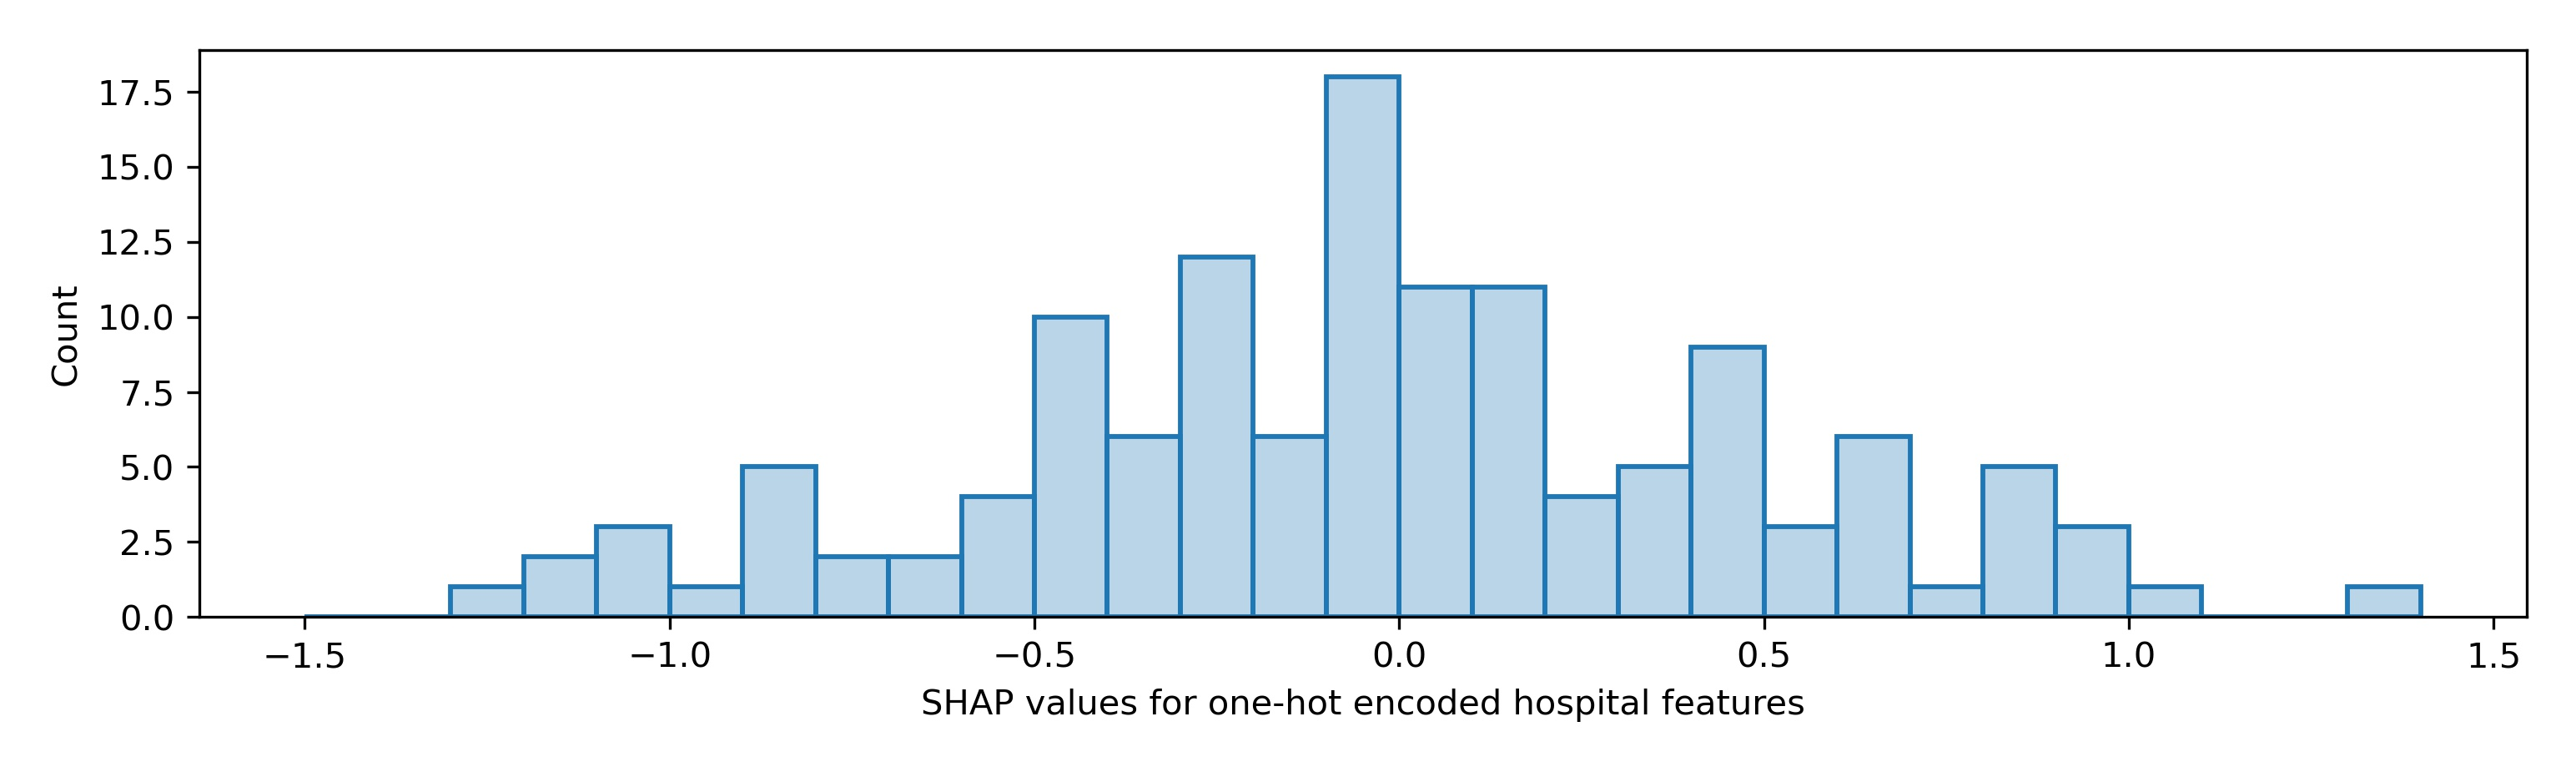
\includegraphics[width=1.0\textwidth]{./images/03d_xgb_10_features_hosp_shap_hist.jpg}
\end{center}
\scriptsize
SHAP effects: \\
$\pm1$: Odds change $\pm3$ fold\\
$\pm2$: Odds change $\pm7$ fold\\
$\pm3$: Odds change $\pm20$ fold\\
$\pm4$: Odds change $\pm55$ fold\\
$\pm5$: Odds change $\pm150$ fold
\end{frame}


%\begin{frame}
\frametitle{We can predict what decision each hospital would make on different patients}

\vspace{3mm}

\begin{columns}[t]
    \begin{column}{0.45\textwidth}
        Base patient:
        \begin{itemize}
            \footnotesize
            \item Onset to arrival = 80 mins
            \item Arrival to scan = 20 mins
            \item Infarction = Yes
            \item NIHSS = 15
            \item Prior disability level = 0
            \item Precise onset time = Yes
            \item Use of AF anticoagulents = No
        \end{itemize}
    \end{column}
    
    \begin{column}{0.5\textwidth}
    \color{teal}
    Proportion of hospitals predicted to give thrombolysis:
    \footnotesize
    \begin{itemize}
        \color{teal}
        \item Base patient: 99\%
    \end{itemize}
    %\pause{} %Creates 2 PDF slides with pause here
    \vspace{3mm}
    \normalfont
    \color{red}
    \normalsize
    Base patient with:
    \footnotesize
    \begin{itemize}
        \color{red}
        \item NIHSS = 4: 73\%
        \item Pre-stroke mRS = 3: 86\%
        \item Estimated stroke onset time: 64\%
    \end{itemize}
    \end{column}

\end{columns}

\vspace{7mm}
This allows us to open up discussions between hospitals on differences in choices around thrombolysis.
\end{frame}

\begin{frame}
\frametitle{Outcome model feature selection}

The outcome model is a multi-level outcome of disability (modified Rankin Scale, mRS) ranging from 0 (no disability) to 6 (death). 

\vspace{2mm}

Pre-stroke mRS is estimated for all patients, and mRS on discharge from inpatient care is recorded for all patients.

\vspace{3mm}

\begin{center}
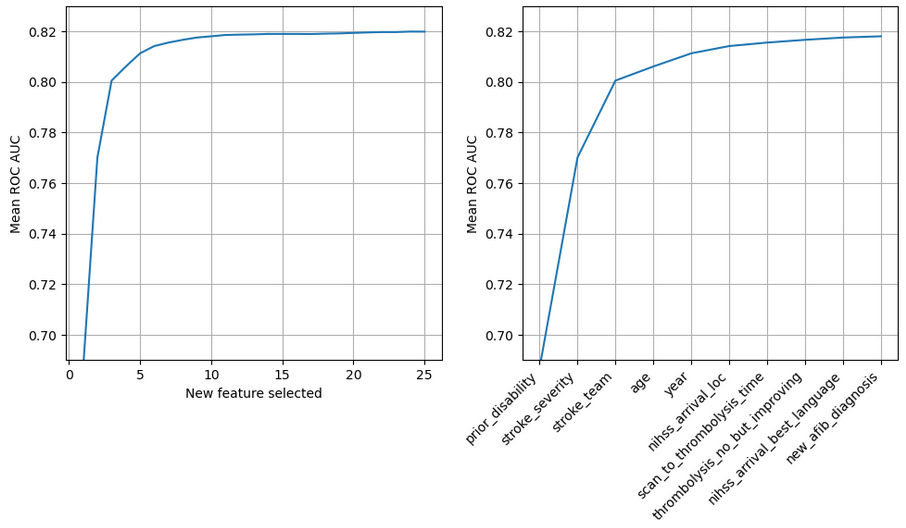
\includegraphics[width=0.85\textwidth]{./images_outcome/outcome_feature_selection}
\end{center}


\end{frame}
\begin{frame}
\frametitle{Outcome model SHAP}

SHAP for odds of a patient being discharged with mRS $\leq$ 2 (no significant disability).


\begin{center}
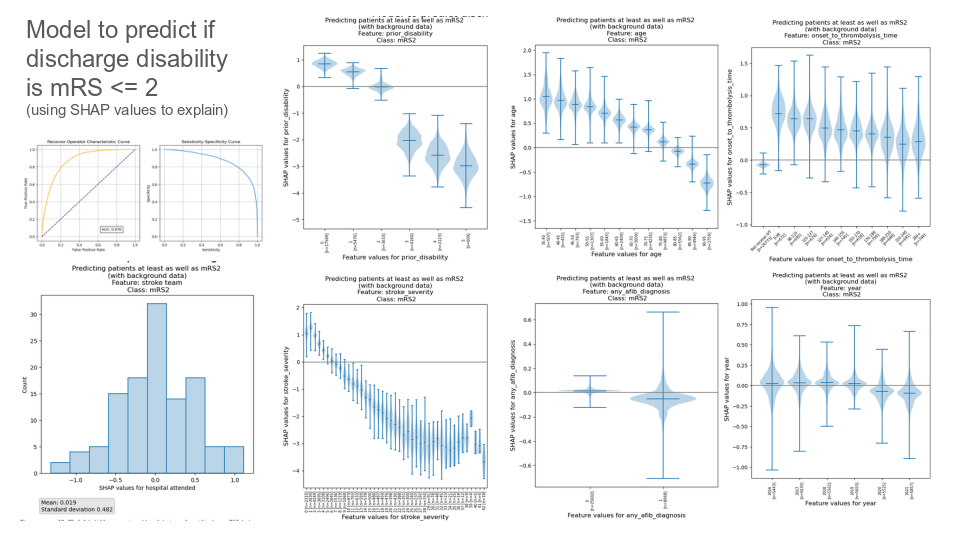
\includegraphics[width=1.01\textwidth]{./images_outcome/stroke_outcome_shap}
\end{center}


\end{frame}
\begin{frame}
\frametitle{But would be the outcome for my patient?}

Machine learning allows personalised prediction of outcomes - so for that same patient, we can predict the probabilities of different levels of disability on discharge, with and without treatment.

\vspace{5mm}

\begin{center}
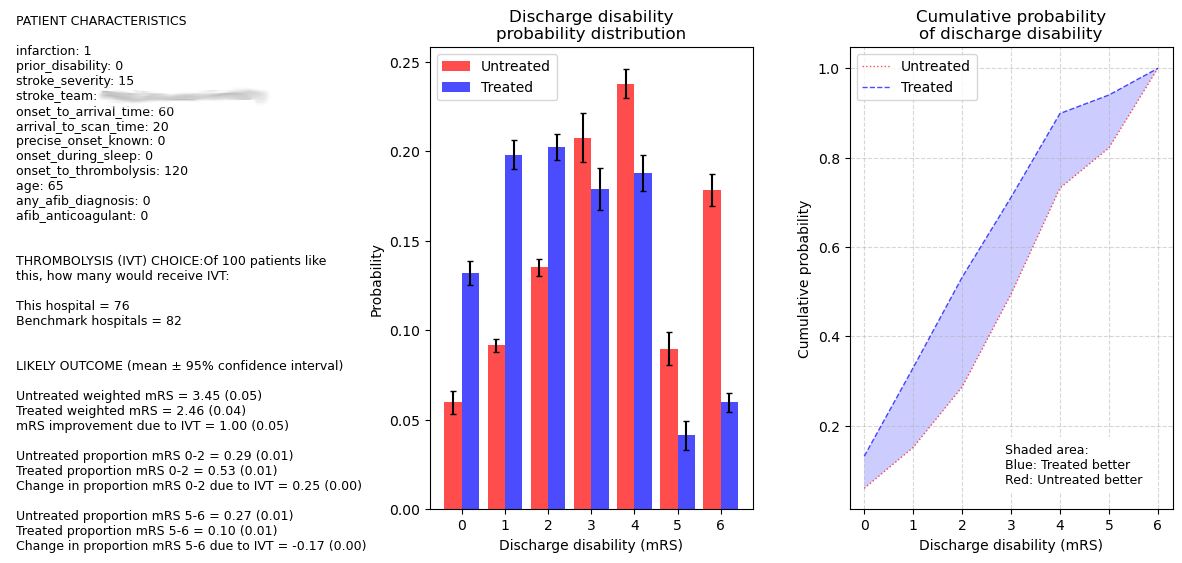
\includegraphics[width=1.0\textwidth]{./images_outcome/full_outcome_1}
\end{center}


\end{frame}

\begin{frame}
\frametitle{But would be the outcome for my patient? Simplified output}

\vspace{5mm}

\begin{center}
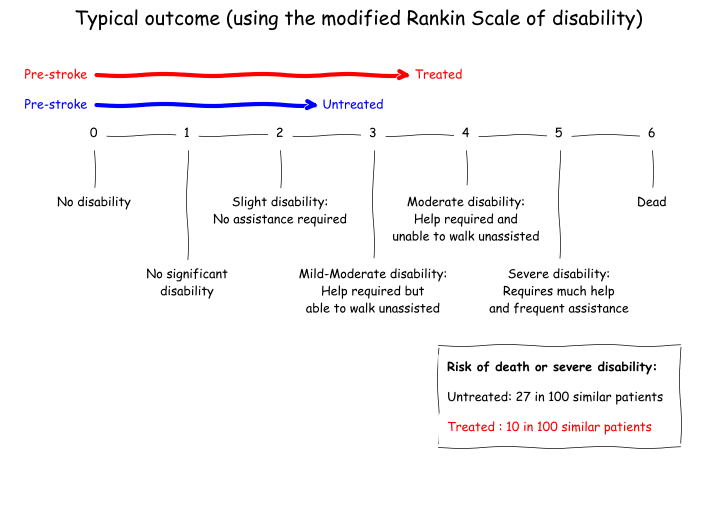
\includegraphics[width=1.0\textwidth]{./images_outcome/short_outcome_1}
\end{center}


\end{frame}

%\begin{frame}
\frametitle{But would be the outcome for my patient? Mild stroke}

Machine learning allows personalised prediction of outcomes - so for that same patient, we can predict the probabilities of different levels of disability on discharge, with and without treatment.

\vspace{5mm}

\begin{center}
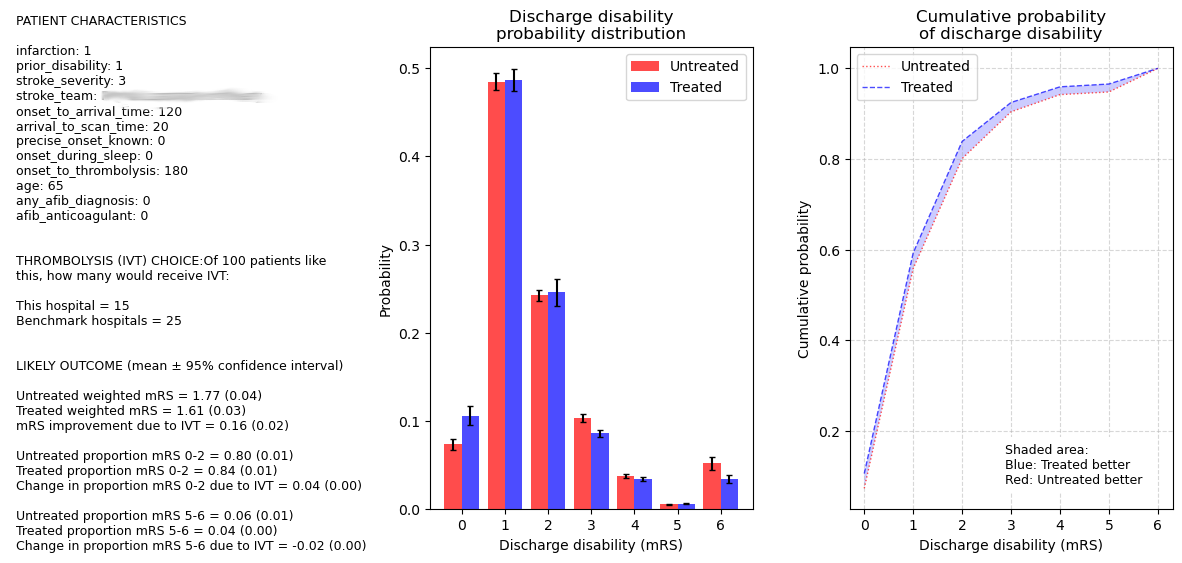
\includegraphics[width=1.0\textwidth]{./images_outcome/full_outcome_2}
\end{center}


\end{frame}

%\begin{frame}
\frametitle{But would be the outcome for my patient? Mild Stroke - Simplified output}

\vspace{5mm}

\begin{center}
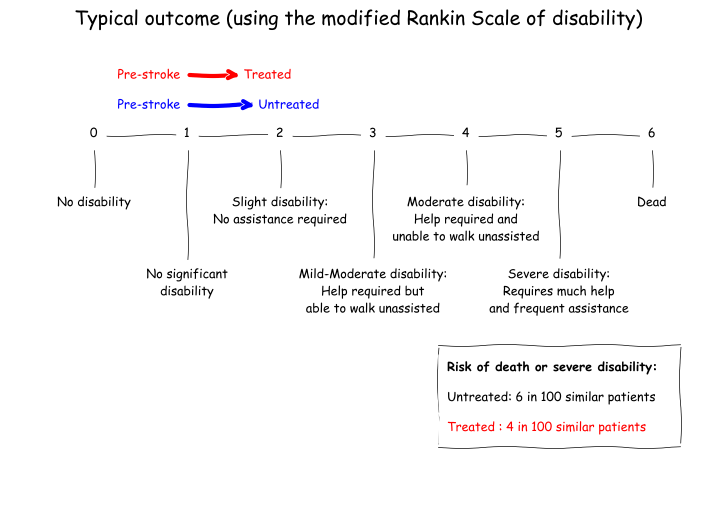
\includegraphics[width=0.9\textwidth]{./images_outcome/short_outcome_2}
\end{center}


\end{frame}

\begin{frame}
\frametitle{Outcome regression analysis}

Using SHAP to estimate the log-odds of improved outcome with thrombolysis allows us to replicate the clinical trials showing the effectiveness of thrombolsysis, and the decline in effectiveness over time.

\vspace{2mm}

The results show that the clinical effectiveness of thrombolysis in real life is as good as the clinical trials predicted (which some have doubted).


\begin{center}
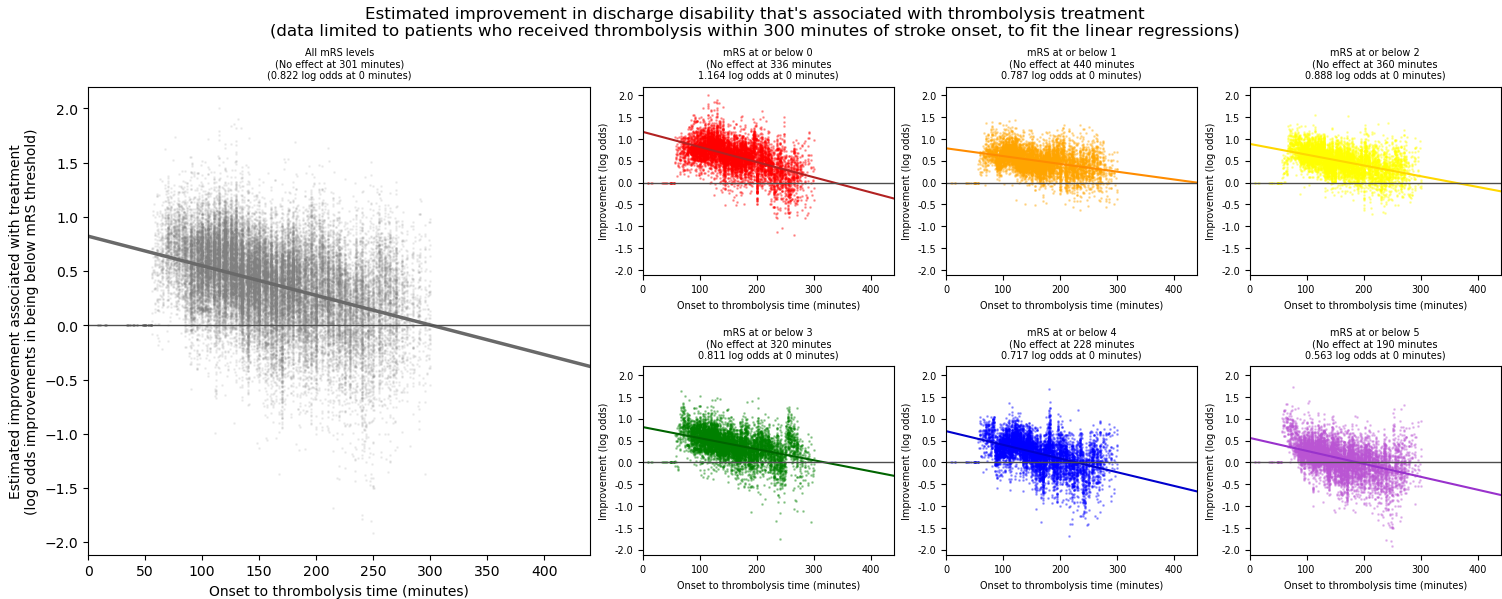
\includegraphics[width=1.01\textwidth]{./images_outcome/outcome_regression}
\end{center}


\end{frame}
\begin{frame}
\frametitle{Full model (anonymised hospital) - pathway simulation + machine learning}

\begin{center}
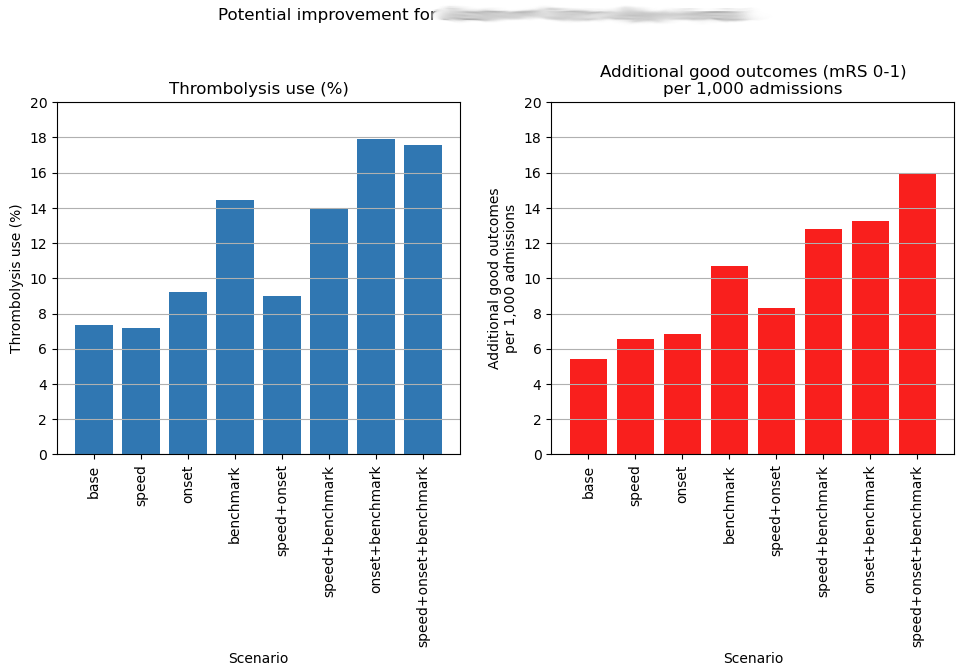
\includegraphics[width=0.8\textwidth]{./images_outcome/hosp_improvement_1}
\end{center}

\footnotesize
Note: Outcomes here are based on a mathematical model based on clinical trials.

\end{frame}

\begin{frame}
\frametitle{Patient subgroups}

\begin{center}
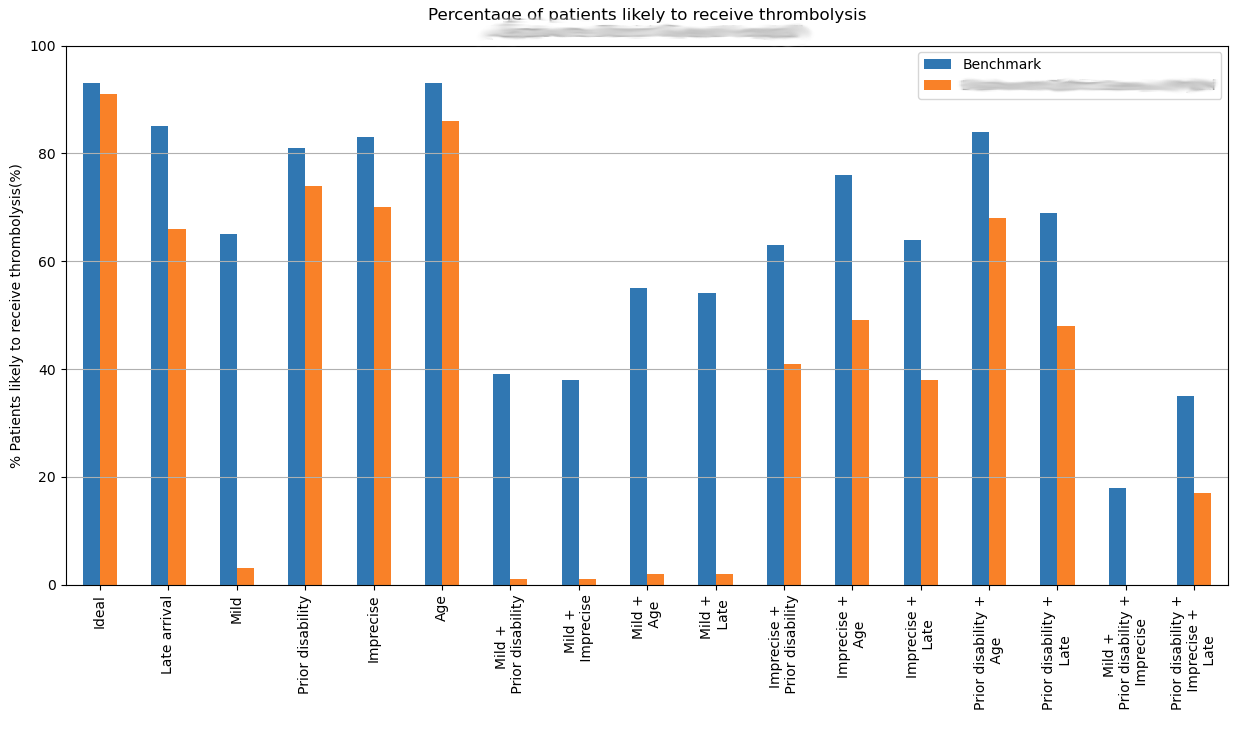
\includegraphics[width=1.0\textwidth]{./images_outcome/hosp_subgroups_1}
\end{center}

\end{frame}




\begin{frame}
\frametitle{Summary}
\small

\begin{itemize}
    \item The decision model revealed that the odds of receiving was most influenced by:
    
    \begin{itemize}
        \item Arrival-to-scan time; Stroke type; Stroke severity; Whether onset time was known precisely or was estimated; Pre-stroke disability; Stroke team; Use of anticoagulants for AF; Onset-to-arrival time
    \end{itemize}

\item The hospital identification (hospital SHAP value) explained 58\% of the variance in between-hospital thrombolysis use. Hospitals with lower thrombolysis use were particularly less likely to give thrombolysis to patients with milder strokes, prior disability, or patients with imprecise onset time.

\item The outcome revealed that outcome was most influenced by:
    
    \begin{itemize}
        \item Prior disability; Stroke severity; Stroke team; Age; Scan-to-thrombolysis time
        \item Note: Whether stroke onset time was known precisely or was estimated influenced choice to use thrombolysis, but did not influence outcomes with/without thrombolysis.
    \end{itemize}

\end{itemize}

\end{frame}

\begin{frame}
\frametitle{Acknowledgements}

\begin{itemize}
    \setlength{\itemsep}{4mm}
    \item \textbf{Kerry Pearn}: Performed most of the work shown here
    \item \textbf{Martin James}: Clinical lead
    \item \textbf{Anna Laws}: Additional analysis and web applications
    \item \textbf{Richard Everson}: Machine learning advice
    \item \textbf{Leon Farmer}: Patient, and lead of Patient \& Carers Involvement group (Penny Thompson, Simon Douglas, John Williams, David Burgess, Iain and Nicky Hancock)
    \item \textbf{Keira Pratt Boyden, Julia Frost, Iain Lang, Cathy Pope}: Qualitative research
    \item \textbf{Tom Monks}: Help with web apps, and general advice
\end{itemize}
\end{frame}


%%%%%%%%%%%%%%%%%%%%%%%%%%%%%%%%%%%%%%%%%%%%%%%%%%%%%%%%%%%%%%%

\end{document}




